\newpage
\chapter{METODE PENELITIAN} \label{Bab III}

\section{Metode Penelitian} \label{III.MetodePenelitian}

\subsection{Alur Penelitian dan Pemilihan Metode} \label{III.AlurPenelitian}
Penelitian ini dilaksanakan melalui beberapa tahapan yang saling berurutan dan berkesinambungan. Tahapan penelitian dimulai dari identifikasi masalah, studi literatur, analisis kebutuhan, pemilihan metode pengembangan sistem, perancangan sistem, implementasi, pengujian, hingga evaluasi hasil. Alur umum penelitian dapat dilihat pada Gambar \ref{fig:3.alurpenelitian}, yang menggambarkan keseluruhan proses pengembangan sistem dari tahap awal hingga tahap akhir.\par

\begin{figure}[H]
	\centering
	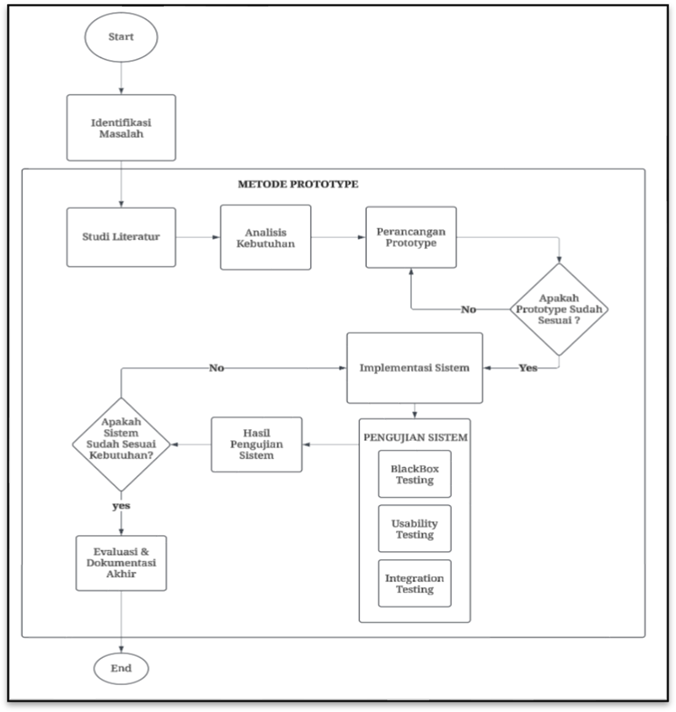
\includegraphics[width=0.85\textwidth]{figure/alur-penelitian.png}
	\caption{Diagram Alur Penelitian}
	\label{fig:3.alurpenelitian}
\end{figure}

Setelah melalui tahap identifikasi masalah dan studi literatur, dilakukan proses pemilihan metode pengembangan sistem yang paling sesuai dengan kebutuhan penelitian.\par

\subsection{Analisis Pemilihan Metode} \label{III.AnalisisPemilihan}
Berdasarkan wawancara dengan pihak Pusat Sistem Informasi Universitas HKBP Nommensen, ditemukan bahwa pengembangan sistem PMB menghadapi kendala pada biaya \textit{hosting}, keterbatasan tenaga pengelola server, serta kebutuhan revisi berulang sebelum sistem siap dipublikasikan. Pihak instansi menyatakan bahwa sistem sebaiknya diselesaikan, diuji, direvisi, dan diuji kembali secara lokal agar efisien dari sisi waktu dan biaya.\par

Dengan kondisi tersebut, metode pengembangan yang bersifat linear dan kaku seperti \textit{Waterfall}, \textit{V-Model}, dan RAD dikeluarkan dari tahap seleksi, karena setiap tahapan harus diselesaikan sepenuhnya sebelum berpindah ke tahap berikutnya. Pendekatan seperti ini tidak menyediakan ruang untuk iterasi tanpa mengulang seluruh proses dari awal.\par

Sementara itu, metode \textit{Agile} (Scrum), meskipun populer dan adaptif menurut literatur, tidak dipilih karena penerapannya menuntut tim besar, pertemuan rutin (\textit{daily sprint}), serta keterlibatan pengguna secara langsung di setiap iterasi---kondisi yang tidak sesuai dengan penelitian individu dan keterbatasan sumber daya institusi.\par

Berdasarkan eliminasi awal, metode yang masih dipertimbangkan adalah \textit{Modified Waterfall}, \textit{Incremental}, dan \textit{Prototype}, karena ketiganya tetap memungkinkan iterasi terbatas dan revisi pada tahap perancangan maupun pengujian. Untuk menentukan metode paling sesuai, dilakukan analisis perbandingan berbasis kriteria lapangan dengan pembobotan seperti pada Tabel \ref{table:3.penilaianmetode}.\par

\begin{longtable}{|p{0.15\textwidth}|p{0.25\textwidth}|p{0.25\textwidth}|p{0.25\textwidth}|}
	\caption{Penilaian Kesesuaian Metode Berdasarkan Kriteria Lapangan}
	\label{table:3.penilaianmetode}\\
	\hline
	\textbf{Kriteria} & \textbf{\textit{Modified Waterfall}} & \textbf{\textit{Incremental}} & \textbf{\textit{Prototype}} \\
	\hline
	\endfirsthead
	\hline
	\textbf{Kriteria} & \textbf{\textit{Modified Waterfall}} & \textbf{\textit{Incremental}} & \textbf{\textit{Prototype}} \\
	\hline
	\endhead
	Fleksibilitas terhadap revisi & 3 -- Revisi hanya dapat dilakukan setelah satu tahap selesai sepenuhnya, sehingga perubahan di tengah proses sulit dilakukan. & 4 -- Dapat menambah fitur baru di versi berikutnya, tetapi sulit mengubah fitur lama karena sudah menjadi dasar modul lain. & 5 -- Setiap versi \textit{prototype} bisa langsung diperbaiki kapan saja tanpa menunggu tahap selesai. \\
	\hline
	Kesesuaian dengan keterbatasan biaya & 3 -- Setiap tahap membutuhkan pengujian terpisah sehingga menambah waktu dan biaya. & 4 -- Cukup efisien karena pengembangan bertahap, tetapi tetap perlu penyebaran per versi. & 5 -- Dapat diuji lokal tanpa perlu \textit{hosting} server, sangat hemat biaya untuk instansi. \\
	\hline
	Kesesuaian dengan pola kerja instansi & 4 -- Proses kerja jelas dan mudah dikontrol, namun revisi mendadak sulit dilakukan. & 3 -- Cocok untuk proyek modular, tetapi tidak mendukung validasi langsung oleh pengguna. & 5 -- Sesuai dengan pola kerja instansi yang membutuhkan revisi cepat setelah setiap uji coba. \\
	\hline
	Kemudahan pengujian berulang & 3 -- Pengujian hanya dilakukan di akhir tahap tertentu, bukan setelah setiap perubahan kecil. & 3 -- Pengujian dilakukan per modul, sulit untuk menguji sistem secara keseluruhan. & 5 -- \textit{Prototype} dapat diuji langsung setelah diperbarui untuk melihat hasil secara instan. \\
	\hline
	Efisiensi waktu dan sumber daya & 4 -- Efisien untuk sistem kecil, tetapi lambat jika banyak revisi diperlukan. & 4 -- Efisien untuk pengembangan modular dengan jadwal tetap. & 4 -- Iterasi memerlukan waktu lebih lama, tetapi hasil lebih akurat dan stabil. \\
	\hline
\end{longtable}

\subsection{Hasil Analisis dan Kesimpulan Pemilihan Metode} \label{III.HasilAnalisis}
Hasil perhitungan menunjukkan bahwa metode \textit{Prototype} memperoleh rata-rata total skor yaitu 4,85 dan yang tertinggi di antara metode lainnya, menandakan kesesuaian paling tinggi terhadap kebutuhan penelitian. Pendekatan ini dianggap optimal karena:\par

\begin{enumerate}[noitemsep]
	\item Fleksibel dan iteratif, memungkinkan revisi cepat berdasarkan hasil pengujian tanpa memulai dari awal.
	\item Efisien secara biaya dan waktu, dapat diuji secara lokal tanpa harus langsung di-\textit{hosting} ke server.
	\item Selaras dengan pola kerja instansi, yang mengutamakan pengujian dan revisi bertahap sebelum implementasi penuh.
	\item Meminimalkan risiko kesalahan besar, karena setiap versi \textit{prototype} diuji dan divalidasi terlebih dahulu.
\end{enumerate}

Dengan demikian, metode \textit{Prototype} dipilih sebagai dasar pengembangan sistem informasi PMB berbasis Spring Framework. Secara lebih spesifik, pendekatan yang digunakan adalah \textit{Evolutionary Prototyping} sebagaimana diuraikan pada Subbab \ref{II.EvolutionaryPrototyping}. Pendekatan ini dipilih karena sistem PMB memiliki banyak modul (pendaftaran, pembayaran, ujian, validasi, daftar ulang, dan lain-lain) yang tidak memungkinkan untuk dibangun seluruhnya dalam satu tahap. Dengan \textit{Evolutionary Prototyping}, \textit{prototype} yang dibangun pada setiap iterasi tidak dibuang, melainkan terus disempurnakan hingga menjadi sistem akhir. Hal ini sesuai dengan kondisi penelitian yang dikerjakan oleh satu pengembang secara bertahap dengan umpan balik langsung dari pihak instansi \cite{crinnion1991evolutionary, davis1992operational}.\par

\section{Penjabaran Alur Penelitian} \label{III.PenjabaranAlur}
Setiap tahapan dalam alur penelitian memiliki peran penting dalam mendukung keberhasilan pengembangan sistem PMB berbasis Spring Framework. Pendekatan \textit{Evolutionary Prototyping} diterapkan dengan membagi pengembangan ke dalam beberapa iterasi, di mana setiap iterasi menghasilkan versi sistem yang fungsional dan dapat dievaluasi. Berikut penjabaran detail dari setiap tahap:\par

\subsection{Identifikasi Masalah} \label{III.IdentifikasiMasalah}
Tahap awal penelitian dilakukan dengan mengamati dan menganalisis permasalahan pada sistem penerimaan mahasiswa baru (PMB) Universitas HKBP Nommensen (UHN). Peneliti melakukan wawancara langsung dengan pihak Pusat Sistem Informasi, yakni Parulian Sirait, M.Kom, selaku \textit{Network Administrator} dan pengelola server yang juga terlibat dalam pengembangan serta pengelolaan website PMB. Beliau menjadi pihak yang sering menerima laporan kendala dari panitia PMB dan calon mahasiswa baru (camaba), termasuk membantu mereka secara langsung melalui WhatsApp dalam proses daftar ulang.\par

Selain itu, dilakukan perbandingan eksternal melalui wawancara dengan pihak PMB Institut Teknologi Sumatera (ITERA) untuk mengukur urgensi dan efisiensi sistem PMB di UHN dibanding kampus lain. Peneliti juga menyebarkan kuesioner daring (Google Form) kepada calon mahasiswa baru dan mahasiswa aktif Prodi Informatika guna mengidentifikasi kendala yang mereka alami saat proses pendaftaran, verifikasi, maupun daftar ulang.\par

\subsection{Studi Literatur} \label{III.StudiLiteratur}
Kajian literatur dilakukan terhadap berbagai referensi ilmiah, jurnal, serta dokumentasi resmi terkait pengembangan aplikasi berbasis Spring Boot, MySQL/PostgreSQL, BRIVA API, dan SMTP. Selain itu, penelitian terdahulu tentang sistem informasi akademik dan metode pengembangan \textit{Prototype} juga menjadi acuan dalam menentukan rancangan serta tahapan sistem PMB yang efisien dan terintegrasi.\par

\subsection{Analisis Kebutuhan} \label{III.AnalisisKebutuhan}
Tahap ini bertujuan memperkuat hasil identifikasi masalah menjadi data yang lebih akurat dan meyakinkan. Pengumpulan data dilakukan melalui wawancara dan kuesioner agar kebutuhan sistem yang dirancang benar-benar sesuai dengan kondisi lapangan.\par

\begin{enumerate}[noitemsep]
	\item \textbf{Wawancara Internal (Pusat Sistem Informasi UHN)}\\
	Peneliti melakukan wawancara langsung (WWC) dengan pihak Pusat Sistem Informasi Universitas HKBP Nommensen, yaitu Bapak Parulian Sirait, M.Kom, selaku \textit{Network Administrator} dan pengelola server PMB. Beliau merupakan pihak yang menangani kendala sistem PMB, menerima laporan dari admin, serta berinteraksi langsung dengan calon mahasiswa melalui WhatsApp terkait daftar ulang. Wawancara ini bertujuan menggali permasalahan sistem lama, alur kerja admin, serta kebutuhan fitur baru pada sistem PMB. Daftar pertanyaan wawancara dapat dilihat di Tabel \ref{table:3.wawancara}.
	
	\item \textbf{Kuesioner Mahasiswa (Calon Mahasiswa Baru dan Mahasiswa Prodi Informatika)}\\
	Selain wawancara, peneliti juga menyebarkan kuesioner daring (Google Form) kepada calon mahasiswa baru tahun berjalan dan mahasiswa aktif Prodi Informatika UHN untuk mengetahui pengalaman pengguna secara langsung terhadap sistem PMB saat ini. Daftar pertanyaan kuesioner dapat dilihat di Tabel \ref{table:3.kuesioner}.
\end{enumerate}

\begin{longtable}{|c|p{0.8\textwidth}|}
	\caption{Daftar Pertanyaan Wawancara dengan Pihak Pusat Sistem Informasi UHN}
	\label{table:3.wawancara}\\
	\hline
	\textbf{No} & \textbf{Pertanyaan} \\
	\hline
	\endfirsthead
	\hline
	\textbf{No} & \textbf{Pertanyaan} \\
	\hline
	\endhead
	1 & Bagaimana alur pendaftaran calon mahasiswa baru dilakukan melalui sistem PMB saat ini? \\
	\hline
	2 & Apakah sistem PMB saat ini sudah terintegrasi dengan sistem akademik atau keuangan universitas? \\
	\hline
	3 & Jika belum terintegrasi, apa kendala utama yang menyebabkan hal tersebut? \\
	\hline
	4 & Bagaimana proses admin dalam memverifikasi data calon mahasiswa dan status pembayaran? \\
	\hline
	5 & Apakah proses verifikasi dan daftar ulang masih dilakukan secara manual oleh admin? \\
	\hline
	6 & Apa dampak dari proses manual tersebut terhadap waktu dan akurasi validasi data? \\
	\hline
	7 & Apakah sistem PMB memiliki fitur notifikasi otomatis kepada calon mahasiswa dan admin? \\
	\hline
	8 & Jika tidak ada, bagaimana pengaruhnya terhadap keterlambatan daftar ulang dan komunikasi? \\
	\hline
	9 & Seberapa besar kesulitan admin dalam memantau seluruh tahapan pendaftaran dari awal hingga daftar ulang karena sistem terpisah? \\
	\hline
	10 & Apakah sering terjadi keterlambatan atau kesalahan input akibat sistem yang belum terhubung antar modul? \\
	\hline
	11 & Bagaimana komunikasi biasanya dilakukan antara admin dan calon mahasiswa ketika terjadi kendala? \\
	\hline
	12 & Menurut Bapak, fitur apa yang paling mendesak untuk diterapkan pada sistem PMB agar lebih efisien dan terintegrasi? \\
	\hline
	13 & Seberapa penting menurut Bapak penerapan sistem PMB terintegrasi berbasis web bagi UHN ke depannya? \\
	\hline
\end{longtable}

\begin{longtable}{|c|p{0.8\textwidth}|}
	\caption{Daftar Pertanyaan Kuesioner Mahasiswa}
	\label{table:3.kuesioner}\\
	\hline
	\textbf{No} & \textbf{Pertanyaan} \\
	\hline
	\endfirsthead
	\hline
	\textbf{No} & \textbf{Pertanyaan} \\
	\hline
	\endhead
	1 & Apakah proses pendaftaran PMB mudah dipahami tanpa harus meminta bantuan admin? \\
	\hline
	2 & Apakah Anda pernah mengalami kesulitan saat mengisi formulir atau mengunggah berkas pendaftaran? \\
	\hline
	3 & Apakah informasi tahapan pendaftaran tersedia secara jelas di website PMB? \\
	\hline
	4 & Apakah Anda pernah mengalami keterlambatan dalam konfirmasi pendaftaran atau pembayaran? \\
	\hline
	5 & Apakah sistem memberikan notifikasi otomatis mengenai status pendaftaran Anda? \\
	\hline
	6 & Jika tidak, apakah Anda harus menghubungi admin secara manual (melalui WhatsApp atau media lain)? \\
	\hline
	7 & Apakah proses daftar ulang berjalan lancar tanpa kesalahan data atau keterlambatan? \\
	\hline
	8 & Apakah tampilan dan navigasi website PMB mudah digunakan di berbagai perangkat (desktop/mobile)? \\
	\hline
	9 & Apa kendala utama yang menurut Anda paling menghambat proses pendaftaran mahasiswa baru di UHN? \\
	\hline
	10 & Seberapa puas Anda terhadap sistem PMB UHN saat ini (skala 1--5)? \\
	\hline
\end{longtable}

\subsection{Perancangan dan Desain Sistem} \label{III.PerancanganPrototype}
Tahap perancangan dilakukan berdasarkan hasil analisis kebutuhan yang diperoleh dari wawancara dan kuesioner. Pada tahap ini, peneliti menyusun rancangan sistem Penerimaan Mahasiswa Baru (PMB) dengan menerapkan konsep arsitektur \textit{Model--View--Controller} (MVC) sebagai kerangka logis. Perancangan dilakukan melalui proses \textit{quick design} dengan pendekatan berorientasi objek (OOP) dan pemodelan menggunakan \textit{Unified Modeling Language} (UML).\par

Hasil dari tahap ini berupa diagram konteks, \textit{use case diagram}, \textit{activity diagram}, \textit{class diagram}, serta rancangan antarmuka sistem. Perancangan ini menjadi dasar bagi seluruh iterasi pengembangan yang akan dilakukan.\par

\subsection{Pengembangan Iteratif (\textit{Evolutionary Prototyping})} \label{III.PengembanganIteratif}
Sesuai dengan pendekatan \textit{Evolutionary Prototyping}, implementasi sistem dilakukan secara bertahap melalui beberapa iterasi. Setiap iterasi menghasilkan versi sistem yang fungsional dan dapat digunakan, bukan sekadar \textit{mockup}. \textit{Prototype} dari iterasi sebelumnya tidak dibuang, melainkan menjadi fondasi bagi iterasi selanjutnya \cite{crinnion1991evolutionary}. Pembagian iterasi didasarkan pada prioritas modul dan kompleksitas fitur, sebagai berikut:\par

\subsubsection{Iterasi 1 -- Modul Inti Pendaftaran dan Pembayaran}
Iterasi pertama berfokus pada pembangunan alur utama sistem yang menjadi fondasi bagi seluruh proses PMB. Modul yang dikembangkan pada iterasi ini meliputi:\par
\begin{enumerate}[noitemsep]
	\item Halaman pemilihan gelombang dan jenis seleksi/formula
	\item Halaman pemilihan metode pembayaran (Virtual Account dan upload manual)
	\item Halaman pembayaran BRIVA dan upload bukti pembayaran manual
	\item Halaman pembayaran cicilan mahasiswa
	\item Pengisian dan pengiriman formulir pendaftaran
	\item Halaman revisi formulir setelah penolakan admin
	\item Halaman profil mahasiswa dan ubah \textit{password}
	\item Mode ujian \textit{online} (Google Form) dan \textit{offline} (upload bukti)
	\item Konfigurasi link ujian \textit{online}/\textit{offline} oleh admin
	\item Verifikasi pembayaran manual dan approval cicilan oleh admin
\end{enumerate}

Pengujian non-fungsional pada Iterasi~1 dilakukan menggunakan \textit{white-box testing} berbasis JaCoCo untuk mengukur cakupan kode (\textit{code coverage}) dari kelas-kelas yang diimplementasikan pada iterasi ini. Metrik yang diukur meliputi \textit{line coverage}, \textit{branch coverage}, dan \textit{method coverage}. Target cakupan minimal yang ditetapkan adalah 70\% untuk \textit{line coverage} dan \textit{branch coverage} pada modul inti.\par

\subsubsection{Iterasi 2 -- Modul Pendukung dan Administrasi}
Iterasi kedua berfokus pada fitur-fitur pendukung, administrasi lanjutan, serta komponen infrastruktur sistem. Modul yang dikembangkan meliputi:\par
\begin{enumerate}[noitemsep]
	\item Manajemen \textit{system links} dan informasi kontak
	\item Modul pengumuman CRUD
	\item Sistem token ujian (\textit{generate} dan validasi)
	\item \textit{Registration status tracker} multi-tahap
	\item Halaman ekspor data (formulir, daftar ulang, hasil akhir)
	\item Fitur \textit{customer service} (\textit{chat widget})
	\item Manajemen akun admin dan pengguna
	\item \textit{Bulk download} PDF dan \textit{bulk initialize}
	\item Komponen UI bersama (\textit{header}, \textit{footer}, \textit{carousel}, \textit{password strength indicator})
	\item \textit{Background task} pengecekan pembayaran dan publikasi hasil otomatis
\end{enumerate}

Pengujian non-fungsional pada Iterasi~2 dilakukan menggunakan \textit{white-box testing} berbasis JaCoCo untuk mengukur cakupan kode dari kelas-kelas yang diimplementasikan pada iterasi ini. Metrik yang diukur meliputi \textit{line coverage}, \textit{branch coverage}, dan \textit{method coverage}. Target cakupan minimal yang ditetapkan adalah 70\% untuk \textit{line coverage} dan \textit{branch coverage} pada modul pendukung dan administrasi.\par

Setiap iterasi melewati siklus: \textbf{build} $\rightarrow$ \textbf{evaluasi pengguna} $\rightarrow$ \textbf{perbaikan} $\rightarrow$ \textbf{iterasi berikutnya}, sebagaimana ditunjukkan pada Gambar \ref{fig:2.evolutionaryprototyping}.\par

\subsection{Pengujian Sistem} \label{III.PengujianSistem}
Pengujian dilakukan di setiap akhir iterasi untuk memastikan kualitas modul yang dibangun, serta secara menyeluruh setelah seluruh iterasi selesai. Pengujian dilakukan melalui empat pendekatan utama, yaitu:\par

\begin{enumerate}[noitemsep]
	\item \textbf{\textit{Black-Box Testing}} -- digunakan untuk menguji fungsionalitas sistem tanpa melihat struktur internal kode. Pengujian ini berfokus pada kesesuaian antara \textit{input} dan \textit{output}, seperti validasi data, proses autentikasi, serta alur transaksi.
	\item \textbf{\textit{Usability Testing} (SUS Method)} -- bertujuan menilai kemudahan penggunaan sistem dari sisi pengguna. Pengujian dilakukan menggunakan metode \textit{System Usability Scale} (SUS) dengan lima skala penilaian, menghasilkan skor yang menggambarkan tingkat kepuasan dan kelayakan sistem dari perspektif pengguna akhir.
	\item \textbf{\textit{Integration Testing}} -- digunakan untuk memastikan bahwa setiap modul atau komponen sistem yang telah diuji secara terpisah dapat saling berinteraksi dengan baik. Pendekatan ini memastikan integrasi antarlapisan seperti \textit{controller}, \textit{service}, \textit{repository}, dan layanan eksternal berjalan sesuai rancangan.
	\item \textbf{\textit{White-Box Testing} (JaCoCo)} -- digunakan untuk mengukur cakupan kode (\textit{code coverage}) pada setiap iterasi sebagai validasi kualitas non-fungsional implementasi. JaCoCo mengukur persentase \textit{line coverage}, \textit{branch coverage}, dan \textit{method coverage} dari kelas yang diuji, dengan target minimal 70\% pada setiap iterasi.
\end{enumerate}

Keempat metode tersebut saling melengkapi: \textit{black-box testing} memastikan sistem berfungsi secara fungsional, \textit{usability testing} menilai pengalaman pengguna, \textit{integration testing} memvalidasi keterpaduan antarmodul, dan \textit{white-box testing} dengan JaCoCo menjamin kualitas cakupan kode secara kuantitatif di setiap iterasi.\par

\subsection{Evaluasi Akhir dan Pemeliharaan} \label{III.Pemeliharaan}
Setelah seluruh iterasi selesai dan pengujian akhir dilakukan, sistem dievaluasi secara menyeluruh untuk menilai kesesuaian dengan tujuan penelitian. Masukan dari pengguna yang diperoleh selama proses iterasi digunakan sebagai dasar penyempurnaan. Sistem yang telah final diterapkan pada lingkungan simulasi atau riil untuk memastikan stabilitas dan keandalannya.\par

\subsection{Dokumentasi dan Penyusunan Laporan} \label{III.Dokumentasi}
Seluruh proses penelitian, mulai dari analisis hingga implementasi di setiap iterasi, didokumentasikan secara sistematis dalam laporan akhir sebagai bentuk pertanggungjawaban ilmiah terhadap hasil pengembangan sistem.\par

\section{Alat dan Bahan} \label{III.AlatBahan}
Penelitian ini memanfaatkan berbagai alat dan bahan yang berfungsi sebagai penunjang dalam proses perancangan dan pengembangan sistem aplikasi Penerimaan Mahasiswa Baru (PMB) berbasis web. Adapun rincian alat dan bahan yang digunakan adalah sebagai berikut:\par

\subsection{Alat} \label{III.Alat}
Alat yang digunakan dalam penelitian ini terdiri dari perangkat keras (\textit{hardware}) dan perangkat lunak (\textit{software}) yang mendukung proses desain, pengembangan, dan pengujian aplikasi:\par

\begin{enumerate}[noitemsep]
	\item \textbf{Perangkat Lunak (\textit{Software}):}
	\begin{enumerate}
		\item Spring Tool Suite (STS) -- sebagai \textit{Integrated Development Environment} (IDE) untuk mengembangkan aplikasi berbasis Spring Boot.
		\item MySQL Workbench / pgAdmin -- untuk pengelolaan dan visualisasi \textit{database} MySQL/PostgreSQL.
		\item Visual Studio Code -- untuk \textit{editing} file HTML/CSS dan dokumentasi ringan.
		\item Edge -- sebagai \textit{browser} utama untuk pengujian sistem.
		\item Gmail SMTP -- untuk layanan pengiriman email secara otomatis dari sistem.
		\item JaCoCo Maven Plugin (\texttt{jacoco-maven-plugin}) -- untuk pengujian \textit{white-box} dan pengukuran cakupan kode (\textit{code coverage}) pada setiap iterasi pengembangan.
	\end{enumerate}
	
	\item \textbf{Perangkat Keras (\textit{Hardware}):}\\
	Perangkat keras yang digunakan untuk menunjang penelitian ini adalah laptop ASUS TUF Gaming F15 dengan spesifikasi sistem operasi Windows 11, prosesor Intel Core i7-11800H, memori 16 GB DDR4, GPU NVIDIA GeForce RTX 3050 Ti, dan penyimpanan SSD berkapasitas 512 GB.
\end{enumerate}

\subsection{Bahan} \label{III.Bahan}
Bahan yang digunakan dalam penelitian ini terdiri dari berbagai data dan dokumen penunjang, baik yang diperoleh dari studi sebelumnya maupun dari institusi terkait. Bahan-bahan tersebut adalah:\par

\begin{enumerate}[noitemsep]
	\item Dokumen Panduan Pendaftaran Mahasiswa Baru -- berupa file PDF dan petunjuk alur pendaftaran resmi yang diperoleh dari hasil wawancara dengan pihak Pusat Sistem Informasi Universitas HKBP Nommensen sebagai dasar perancangan sistem.
	\item Referensi Penelitian Sebelumnya -- berupa jurnal dan artikel ilmiah terkait pengembangan sistem PMB menggunakan Laravel, Spring Boot, serta studi perbandingan arsitektur.
	\item Standar Format Data -- seperti struktur formulir pendaftaran, informasi jadwal gelombang, dan format pengiriman notifikasi.
	\item Data Simulasi Pengguna -- berupa \textit{dummy data} calon mahasiswa untuk kebutuhan pengujian fitur sistem seperti pendaftaran, login, dan pembayaran.
	\item Template Email Notifikasi -- untuk kebutuhan pengujian pengiriman email menggunakan protokol SMTP Gmail.
\end{enumerate}

\section{Analisis Kebutuhan Sistem} \label{III.AnalisisKebutuhanSistem}

\subsection{Kebutuhan Fungsional} \label{III.KebutuhanFungsional}

\begin{longtable}{|p{0.1\textwidth}|p{0.2\textwidth}|p{0.6\textwidth}|}
	\caption{Kebutuhan Fungsional}
	\label{table:3.kebutuhanfungsional}\\
	\hline
	\textbf{ID} & \textbf{Kebutuhan} & \textbf{Penjelasan} \\
	\hline
	\endfirsthead
	\hline
	\textbf{ID} & \textbf{Kebutuhan} & \textbf{Penjelasan} \\
	\hline
	\endhead
	PMB01-F002 & Pengelolaan periode penerimaan & Admin pusat dapat menambah, mengedit, dan menghapus periode pendaftaran beserta tanggal mulai dan akhir pendaftaran. \\
	\hline
	PMB01-F003 & Penentuan jenis seleksi per periode & Admin pusat dapat menentukan jenis seleksi di setiap periode (bebas testing, bebas testing dengan syarat ranking, atau testing). \\
	\hline
	PMB01-F004 & Penentuan harga formulir & Admin pusat menetapkan harga formulir pendaftaran berdasarkan jenis jalur dan perbedaan antara fakultas kedokteran dan non-kedokteran. \\
	\hline
	PMB01-F005 & Pengelolaan informasi terbaru & Admin pusat mengelola konten pada halaman utama seperti jadwal dan informasi umum, serta mengelola modul pengumuman dengan operasi CRUD (\textit{Create}, \textit{Read}, \textit{Update}, \textit{Delete}). \\
	\hline
	PMB01-F007 & Pengaturan \textit{link} ujian & Admin pusat dapat mengubah tautan ujian (Google Form atau ujian \textit{offline}) dan mengelola token ujian yang akan digunakan oleh camaba. \\
	\hline
	PMB01-F008 & Pengelolaan konten daftar ulang & Admin pusat mengatur isi dan pengumuman daftar ulang yang akan muncul di halaman camaba. \\
	\hline
	PMB01-F009 & Penjadwalan publikasi hasil kelulusan & Admin pusat menentukan waktu publikasi hasil kelulusan, baik per periode maupun secara serentak. \\
	\hline
	PMB01-F010 & Manajemen akun pengguna & Admin pusat dapat menambah atau menghapus akun admin pusat, admin validasi, dan camaba. \\
	\hline
	PMB01-F011 & Penetapan tarif cicilan per program studi & Admin pusat menetapkan nominal cicilan berdasarkan program studi yang dipilih. Admin validasi dapat menyetujui atau menolak permintaan cicilan dari camaba. \\
	\hline
	PMB01-F012 & Aktivasi \textit{virtual account} berdasarkan cicilan dan prodi & Sistem menentukan total pembayaran VA sesuai jumlah cicilan dan program studi. Camaba dapat memilih jumlah cicilan dan memantau status persetujuan serta pembayaran cicilan. \\
	\hline
	PMB01-F013 & Penayangan status kelulusan sesuai waktu & Sistem menampilkan hasil kelulusan hanya pada waktu yang telah dijadwalkan. \\
	\hline
	PMB01-F015 & Email notifikasi \textit{virtual account} & Sistem mengirim email otomatis berisi detail VA dan panduan pembayaran. \\
	\hline
	PMB01-F016 & Halaman informasi \textit{virtual account} & Sistem menampilkan informasi VA, nominal, tenggat waktu, dan panduan pembayaran. \\
	\hline
	PMB01-F017 & \textit{Generate} dan verifikasi pembayaran BRIVA & Sistem membuat nomor VA untuk setiap camaba dan memverifikasi pembayaran melalui API BRIVA. \\
	\hline
	PMB01-F018 & Pembuatan kartu ujian otomatis & Setelah formulir dikirim, sistem otomatis menghasilkan kartu ujian yang bisa diunduh. \\
	\hline
	PMB01-F019 & Email hasil ujian dan nomor pendaftaran & Jika dinyatakan lulus, sistem mengirimkan nomor pendaftaran dan panduan daftar ulang melalui email. \\
	\hline
	PMB01-F020 & Notifikasi sistem & Sistem memberikan notifikasi kepada camaba terkait status kelulusan, pengisian data, dan aktivasi VA. \\
	\hline
	PMB01-F021 & Akses ujian melalui token & Sistem memvalidasi token ujian yang di-\textit{generate} admin dan menampilkan halaman ujian berisi Google Form dalam \textit{iframe} atau opsi unggah bukti ujian \textit{offline}. \\
	\hline
	PMB01-F022 & Validasi token ujian sebelum akses ujian & Sistem memverifikasi token ujian sebelum mengizinkan akses ke halaman ujian. \\
	\hline
	PMB01-F023 & Validasi oleh admin validasi & Sistem menampilkan daftar camaba yang perlu divalidasi oleh admin validasi. \\
	\hline
	PMB01-F024 & Pembatasan akses data diri & Camaba tidak dapat mengedit data diri setelah formulir dikirim, kecuali jika ditolak oleh admin validasi. \\
	\hline
	PMB01-F027 & \textit{Generate} VA manual & Admin validasi dapat membuat VA manual jika proses otomatis gagal, dengan memasukkan nominal biaya secara manual. \\
	\hline
	PMB01-F028 & Validasi berkas jalur ranking & Admin validasi memeriksa bukti ranking yang diunggah oleh camaba jalur bebas testing dengan syarat ranking. \\
	\hline
	PMB01-F029 & Akses data peserta ujian & Admin validasi dapat melihat dan mengekspor daftar peserta ujian. \\
	\hline
	PMB01-F030 & Akses data camaba lulus & Admin validasi dapat melihat data camaba yang sudah melakukan pembayaran dan pendaftaran ulang. \\
	\hline
	PMB01-F031 & Klasifikasi data berdasarkan fakultas dan prodi & Sistem menampilkan data camaba terkelompok berdasarkan fakultas dan program studi. \\
	\hline
	PMB01-F032 & Ekspor data camaba & Data camaba yang telah lengkap dan terverifikasi dapat diekspor dalam format CSV, JSON, atau dicetak langsung. Admin juga dapat mengunduh dokumen PDF camaba secara massal (\textit{bulk download}). \\
	\hline
	PMB01-F033 & Penolakan data diri camaba & Admin validasi dapat menolak data yang belum lengkap disertai alasan penolakan, dan camaba dapat merevisi formulir melalui halaman revisi khusus yang menampilkan data sebelumnya. \\
	\hline
	PMB01-F034 & Pesan ke camaba & Admin validasi dapat mengirim pesan langsung ke email atau notifikasi sistem camaba. \\
	\hline
	PMB01-F035 & Menjawab pertanyaan camaba & Semua admin validasi dapat membalas pertanyaan camaba dan melihat status pesan yang belum dijawab. \\
	\hline
	PMB01-F040 & Pembuatan akun camaba & Camaba dapat membuat akun baru, satu email hanya untuk satu akun. \\
	\hline
	PMB01-F041 & Lupa \textit{password} atau \textit{username} & Camaba dapat menggunakan fitur pemulihan akun melalui email. \\
	\hline
	PMB01-F042 & Login \textit{multi-level} & Admin pusat, admin validasi, dan camaba dapat login sesuai hak aksesnya. \\
	\hline
	PMB01-F043 & Pembelian formulir dan VA & Camaba dapat memilih gelombang, memilih jenis seleksi (formula) melalui halaman pilihan yang menampilkan detail harga dan deskripsi, mengisi formulir pendaftaran, dan melakukan pembayaran sesuai jalur yang dipilih. \\
	\hline
	PMB01-F044 & Pengiriman pertanyaan & Camaba dapat mengirim pertanyaan kepada admin melalui sistem. \\
	\hline
	PMB01-F045 & Mengikuti ujian & Camaba yang telah membeli formulir dapat mengikuti ujian sesuai jadwal dengan memasukkan token ujian yang di-\textit{generate} oleh admin, kemudian mengerjakan soal melalui Google Form atau mengunggah bukti ujian \textit{offline}. \\
	\hline
	PMB01-F046 & Halaman pendaftaran ulang & Camaba yang lulus dapat masuk ke halaman pendaftaran ulang untuk melengkapi berkas yang diperlukan. \\
	\hline
	PMB01-F047 & Pengisian formulir & Camaba dapat mengisi formulir pendaftaran awal maupun ulang, termasuk pengunggahan berkas untuk jalur ranking. \\
	\hline
\end{longtable}

\subsection{Kebutuhan Non-Fungsional} \label{III.KebutuhanNonFungsional}

\begin{longtable}{|p{0.1\textwidth}|p{0.15\textwidth}|p{0.65\textwidth}|}
	\caption{Kebutuhan Non-Fungsional}
	\label{table:3.kebutuhannonfungsional}\\
	\hline
	\textbf{ID} & \textbf{Parameter} & \textbf{Kebutuhan} \\
	\hline
	\endfirsthead
	\hline
	\textbf{ID} & \textbf{Parameter} & \textbf{Kebutuhan} \\
	\hline
	\endhead
	KKR04-NF01 & \textit{Availability} & Sistem dapat diakses pengguna selama 24 jam penuh. \\
	\hline
	KKR04-NF02 & \textit{Ergonomy} & Tampilan dirancang menarik, rapi, dan mudah digunakan. \\
	\hline
	KKR04-NF04 & \textit{Portability} & Kompatibel dengan berbagai jenis perangkat. \\
	\hline
	KKR04-NF05 & \textit{Security} & Menolak \textit{input} ID atau \textit{password} yang salah saat login. \\
	\hline
	KKR04-NF06 & \textit{Scalability} & Mampu diperluas untuk menangani peningkatan jumlah pengguna. \\
	\hline
	KKR04-NF07 & \textit{Response Time} & Pembaruan data berlangsung maksimal 6 detik. \\
	\hline
	KKR04-NF08 & \textit{Response Time} & Kode unik dikirim kurang dari 30 detik setelah konfirmasi selesai. \\
	\hline
	KKR04-NF09 & \textit{Response Time} & Perpindahan halaman terjadi tidak lebih dari 3 detik. \\
	\hline
	KKR04-NF10 & \textit{Real Time Update} & Sub sistem dapat melakukan pembaruan secara \textit{real time} ketika terjadi pembaruan data. \\
	\hline
\end{longtable}

\subsection{Karakteristik Pengguna} \label{III.KarakteristikPengguna}

\begin{longtable}{|p{0.12\textwidth}|p{0.4\textwidth}|p{0.38\textwidth}|}
	\caption{Karakteristik Pengguna}
	\label{table:3.karakteristikpengguna}\\
	\hline
	\textbf{Kategori Pengguna} & \textbf{Tugas / Fungsi} & \textbf{Hak Akses ke Aplikasi} \\
	\hline
	\endfirsthead
	\hline
	\textbf{Kategori Pengguna} & \textbf{Tugas / Fungsi} & \textbf{Hak Akses ke Aplikasi} \\
	\hline
	\endhead
	Camaba & -- Membuat akun dan login\newline -- Memilih gelombang dan jenis formulir (seleksi)\newline -- Mengisi formulir pendaftaran dan mengunggah berkas\newline -- Melakukan pembayaran melalui BRIVA atau upload manual\newline -- Mencetak kartu ujian dan mengikuti ujian\newline -- Melihat status kehadiran, nilai, dan hasil kelulusan\newline -- Melengkapi data daftar ulang & -- Akses ke halaman pendaftaran, pembayaran, ujian, dan daftar ulang\newline -- Fitur cetak kartu ujian \\
	\hline
	Admin Pusat & -- Menentukan jumlah gelombang, syarat ujian, dan tanggal penting\newline -- Mengelola informasi publik dan pengumuman (CRUD)\newline -- Mengelola program studi (kode, nama, tipe, harga, status)\newline -- Menyusun serta mengumumkan hasil kelulusan\newline -- Menentukan waktu publikasi hasil ujian\newline -- Mengelola akun admin pusat, admin validasi, dan camaba & -- Akses penuh ke panel administrasi pusat\newline -- Manajemen konfigurasi sistem dan struktur data\newline -- Kontrol proses seleksi dan publikasi kelulusan\newline -- Pengelolaan akun pengguna sistem lainnya \\
	\hline
	Admin Validasi & -- Melakukan validasi data daftar ulang camaba\newline -- Menyetujui atau menolak permintaan cicilan camaba\newline -- Melihat dan mengekspor data camaba berdasarkan fakultas dan program studi\newline -- Mengunduh dokumen PDF camaba secara massal & -- Akses ke daftar ulang camaba dan data ujian\newline -- Validasi serta klasifikasi data berdasarkan fakultas/prodi\newline -- Manajemen cicilan dan ekspor data \\
	\hline
\end{longtable}

\section{Perancangan Sistem} \label{III.PerancanganSistem}

\subsection{Rancangan Arsitektur MVC Sistem PMB} \label{III.ArsitekturMVC}

\begin{figure}[H]
	\centering
	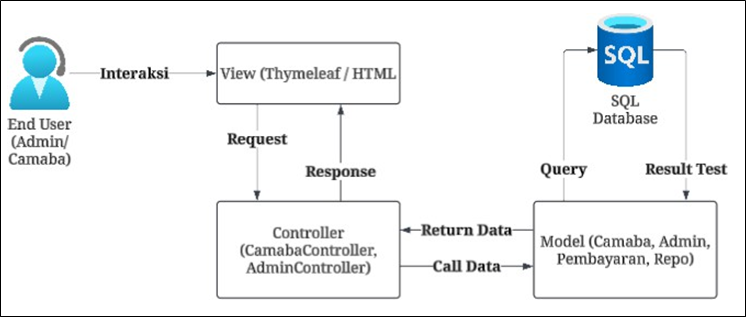
\includegraphics[width=0.85\textwidth]{figure/arsitektur-mvc.png}
	\caption{Diagram Arsitektur MVC}
	\label{fig:3.arsitekturmvc}
\end{figure}

Gambar \ref{fig:3.arsitekturmvc} menampilkan arsitektur \textit{Model-View-Controller} (MVC) yang diterapkan pada sistem Penerimaan Mahasiswa Baru berbasis Spring Boot. Pola ini digunakan untuk memisahkan antara tampilan, pengendali logika, dan pengelolaan data agar pengembangan sistem menjadi lebih teratur, mudah dirawat, serta terbuka untuk pengembangan selanjutnya.\par

Pada sistem ini, pengguna yang terdiri dari admin dan calon mahasiswa baru berinteraksi melalui antarmuka web menggunakan Thymeleaf atau HTML. Setiap tindakan seperti login, pendaftaran, dan validasi pembayaran dikirim sebagai permintaan dari tampilan menuju lapisan pengendali.\par

Bagian \textit{Controller} (misalnya \texttt{CamabaController} dan \texttt{AdminController}) berfungsi menerima permintaan dari pengguna, lalu meneruskannya ke bagian yang menangani logika bisnis di \textit{Model} atau \textit{Service Layer}. \textit{Model} berperan sebagai penghubung antara pengendali dan basis data, berisi struktur data, entitas, serta repositori yang digunakan untuk menjalankan perintah \textit{query}. Misalnya, \texttt{Camaba Model} mengelola data pendaftaran mahasiswa baru, sedangkan \texttt{Pembayaran Model} memproses transaksi dan validasi BRIVA.\par

Alur proses sistem dimulai dari pengguna yang berinteraksi dengan tampilan, kemudian permintaan dikirim ke \textit{Controller}. Setelah itu, \textit{Controller} memanggil fungsi yang diperlukan pada \textit{Model} untuk memproses atau mengambil data dari basis data SQL. Hasilnya dikembalikan ke \textit{Controller}, lalu diteruskan ke tampilan untuk disajikan kembali kepada pengguna.\par

Penerapan arsitektur ini membuat sistem PMB lebih mudah dikelola karena setiap komponen memiliki tanggung jawab yang jelas. Selain itu, struktur ini mendukung integrasi layanan tambahan seperti BRIVA API untuk pembayaran dan SMTP Gmail untuk pengiriman notifikasi secara otomatis, sehingga sistem dapat berjalan secara efisien dan terkoordinasi.\par

\subsection{\textit{Use Case} Diagram} \label{III.UseCaseDiagram}

\begin{figure}[H]
	\centering
	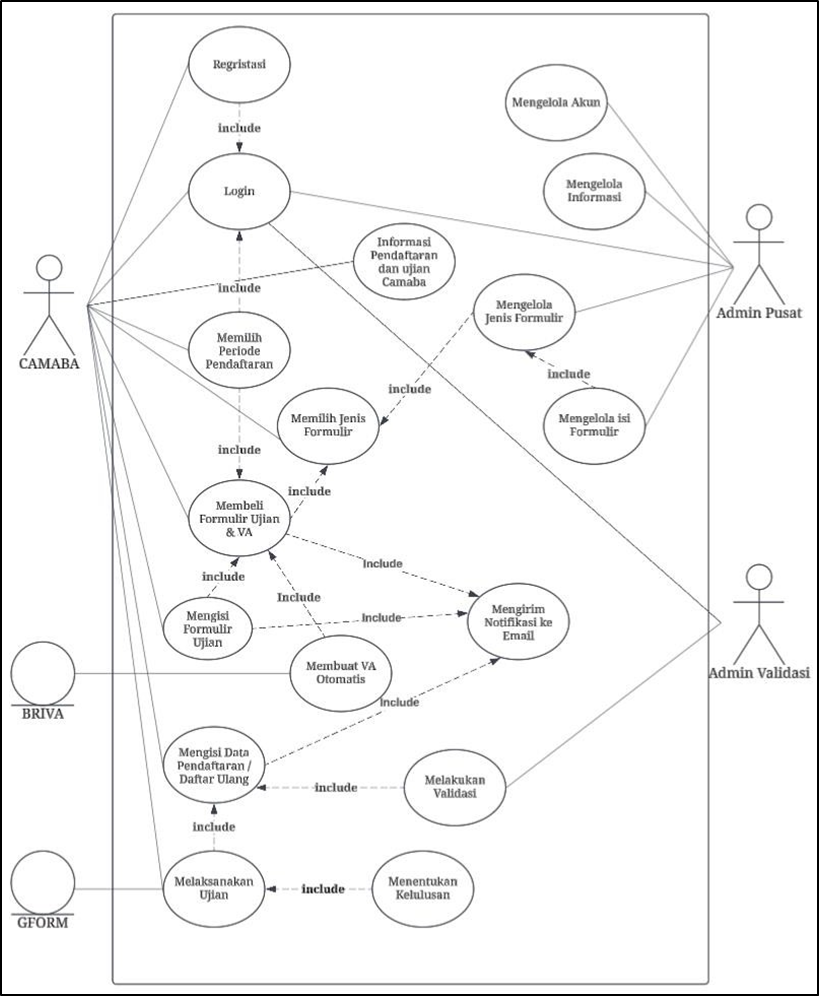
\includegraphics[width=0.85\textwidth]{figure/use-case-diagram.png}
	\caption{Diagram \textit{Use Case}}
	\label{fig:3.usecasediagram}
\end{figure}

\subsubsection{Definisi Aktor}

\begin{longtable}{|p{0.15\textwidth}|p{0.75\textwidth}|}
	\caption{Definisi Aktor \textit{Use Case}}
	\label{table:3.definisiaktor}\\
	\hline
	\textbf{Aktor} & \textbf{Deskripsi} \\
	\hline
	\endfirsthead
	\hline
	\textbf{Aktor} & \textbf{Deskripsi} \\
	\hline
	\endhead
	CAMABA & Aktor utama yang merupakan calon mahasiswa baru. Dapat melakukan registrasi akun, login, memilih dan mengisi formulir pendaftaran, melakukan pembayaran, mengikuti ujian, serta melakukan daftar ulang setelah dinyatakan lulus. \\
	\hline
	Admin Validasi & Bertugas melakukan validasi data pendaftaran CAMABA, mengelola data pendaftaran, memvalidasi ujian, dan memberikan konfirmasi kelulusan kepada CAMABA. \\
	\hline
	Admin Pusat & Memiliki akses penuh untuk mengelola seluruh sistem PMB, termasuk periode pendaftaran, jenis formulir, informasi halaman utama, dan konfigurasi sistem. \\
	\hline
\end{longtable}

\subsubsection{Definisi \textit{Use Case}}

\begin{longtable}{|p{0.2\textwidth}|p{0.7\textwidth}|}
	\caption{Definisi \textit{Use Case}}
	\label{table:3.definisiusecase}\\
	\hline
	\textbf{\textit{Use Case}} & \textbf{Deskripsi} \\
	\hline
	\endfirsthead
	\hline
	\textbf{\textit{Use Case}} & \textbf{Deskripsi} \\
	\hline
	\endhead
	Registrasi & Proses pembuatan akun baru oleh CAMABA dengan mengisi data diri untuk mendapatkan akses ke sistem PMB. \\
	\hline
	Login & Seluruh pengguna sistem harus melakukan login terlebih dahulu untuk mengakses fitur sesuai hak aksesnya. \\
	\hline
	Informasi Pendaftaran dan Ujian CAMABA & Menyediakan informasi lengkap mengenai tahapan pendaftaran, persyaratan, serta jadwal ujian bagi CAMABA. \\
	\hline
	Mengelola Informasi & Admin Pusat dapat menambah, mengubah, atau menghapus informasi pada halaman utama sistem PMB. \\
	\hline
	Memilih Periode Pendaftaran & CAMABA memilih periode pendaftaran yang sedang aktif sebelum memulai proses pendaftaran. \\
	\hline
	Memilih Jenis Formulir & CAMABA menentukan jenis formulir sesuai dengan jalur masuk atau program studi yang dipilih. \\
	\hline
	Mengelola Jenis Formulir & Admin Pusat mengatur daftar jenis formulir yang tersedia di sistem PMB. \\
	\hline
	Membeli Formulir Ujian \& VA & CAMABA membeli formulir ujian yang secara otomatis menghasilkan nomor \textit{virtual account} (VA) untuk pembayaran. \\
	\hline
	Membuat VA Otomatis & Sistem secara otomatis membuat \textit{virtual account} melalui integrasi dengan BRIVA saat CAMABA melakukan pembelian formulir. \\
	\hline
	Membuat VA Manual & Admin membuat \textit{virtual account} secara manual apabila proses otomatis mengalami kendala. \\
	\hline
	Mengisi Formulir Ujian & CAMABA mengisi formulir ujian secara daring dengan data yang sesuai ketentuan. \\
	\hline
	Mengisi Data Pendaftaran / Daftar Ulang & CAMABA melengkapi data pendaftaran setelah dinyatakan lulus seleksi ujian. \\
	\hline
	Melakukan Validasi & Admin Validasi memeriksa dan memverifikasi data pendaftaran CAMABA. Jika valid, sistem mengirimkan notifikasi hasil validasi ke email CAMABA. \\
	\hline
	Mengirim Notifikasi ke Email & Sistem secara otomatis mengirimkan notifikasi email kepada CAMABA terkait hasil validasi atau status pendaftaran. \\
	\hline
	Melaksanakan Ujian & CAMABA mengikuti ujian melalui sistem dengan memasukkan token ujian yang di-\textit{generate} oleh admin, kemudian mengerjakan soal melalui Google Form atau mengunggah bukti ujian \textit{offline}. \\
	\hline
	Menentukan Kelulusan & Admin melakukan verifikasi hasil ujian yang di-\textit{submit} oleh mahasiswa dan menentukan status kelulusan. \\
	\hline
\end{longtable}

\subsection{\textit{Activity} Diagram} \label{III.ActivityDiagram}

\subsubsection{Login Camaba}

\begin{figure}[H]
	\centering
	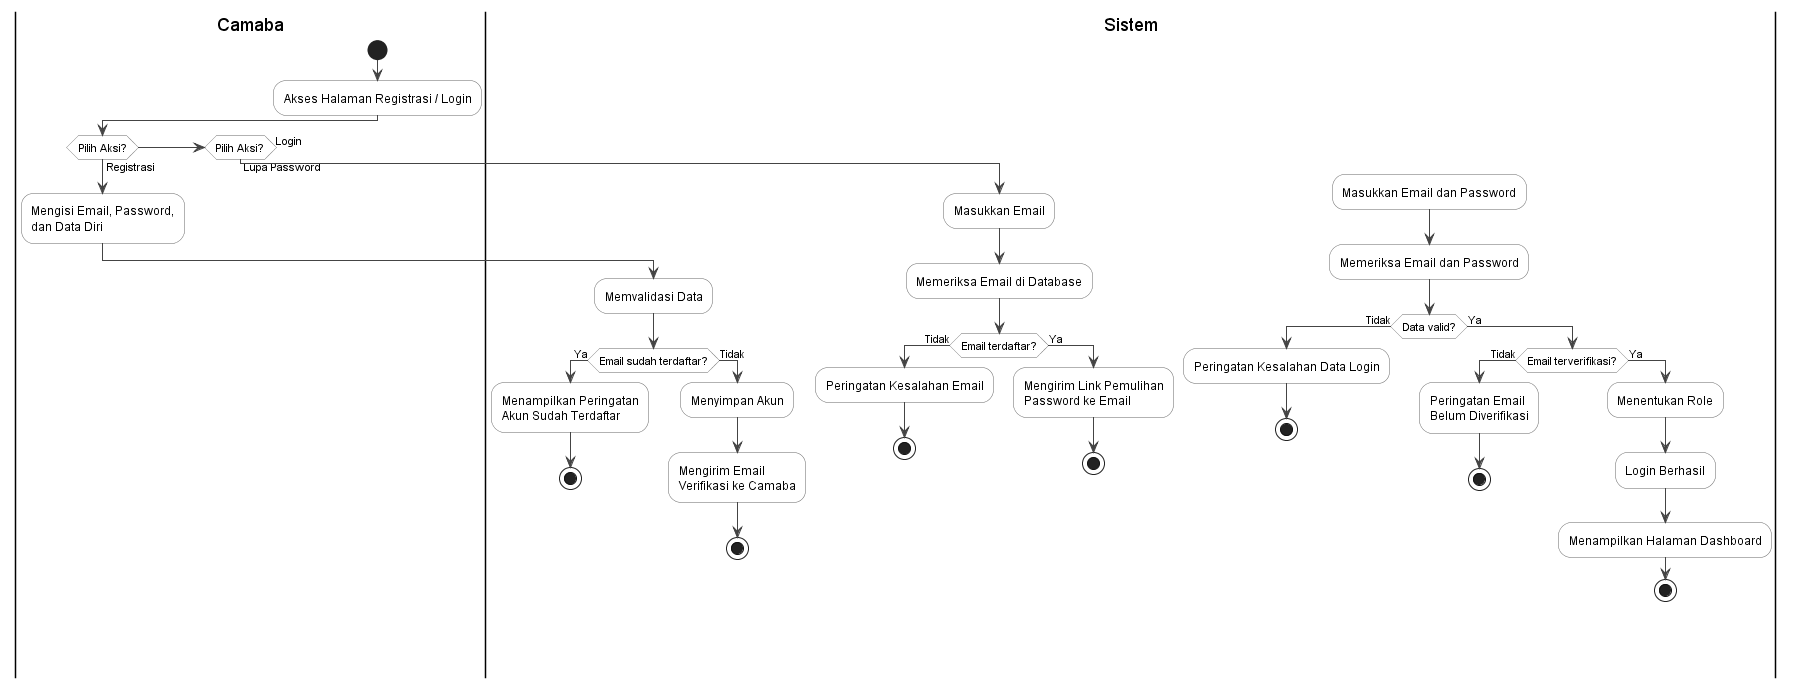
\includegraphics[width=0.85\textwidth]{figure/activity-login-camaba.png}
	\caption{\textit{Activity} Diagram Login Camaba}
	\label{fig:3.activitylogin}
\end{figure}

Saat calon mahasiswa membuka halaman login sistem PMB, sistem menampilkan form untuk memasukkan email dan kata sandi. Jika belum memiliki akun, pengguna dapat melakukan registrasi dengan mengisi data diri. Apabila lupa kata sandi, sistem akan memverifikasi email dan mengirim tautan pemulihan ke Gmail. Setelah login, sistem memeriksa kecocokan data. Jika tidak valid, muncul peringatan kesalahan; jika benar, sistem menentukan \textit{role} pengguna dan menampilkan halaman \textit{dashboard} sesuai hak akses masing-masing.\par

\subsubsection{Registrasi dan Pembelian Formulir PMB UHN}

\begin{figure}[H]
	\centering
	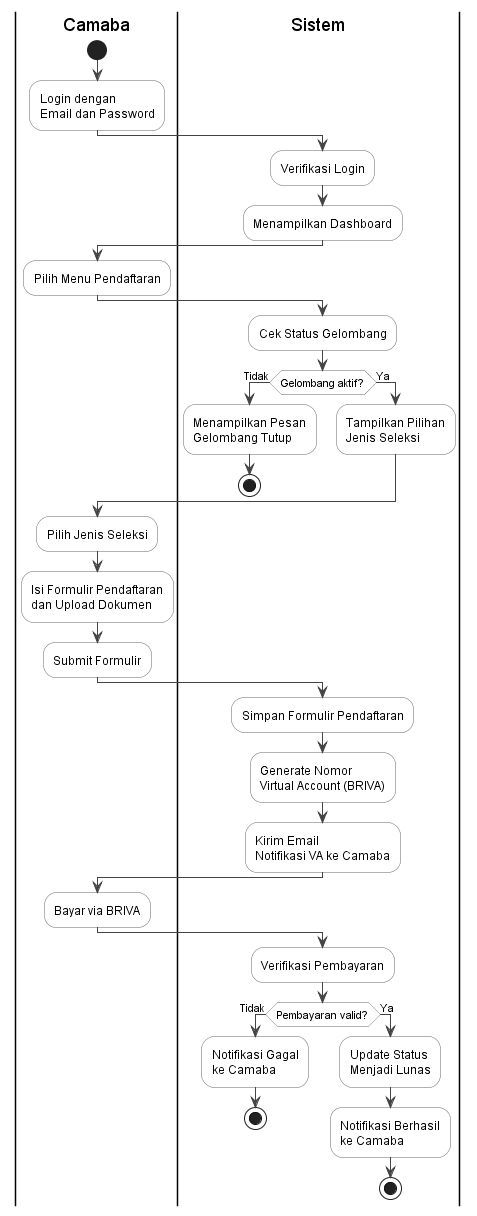
\includegraphics[width=0.85\textwidth]{figure/activity-pembayaran-formulir.png}
	\caption{\textit{Activity} Diagram Pembayaran Formulir Camaba}
	\label{fig:3.activitypembayaran}
\end{figure}

Proses dimulai ketika calon mahasiswa melakukan login ke sistem PMB. Setelah data login diverifikasi, sistem menentukan \textit{role} pengguna dan menampilkan halaman \textit{dashboard}. Dari sana, pengguna memilih menu pendaftaran dan menentukan gelombang yang diinginkan. Sistem kemudian memeriksa status gelombang, apakah masih aktif atau sudah ditutup. Jika masih aktif, pengguna memilih jenis formulir (jenis seleksi) yang tersedia.\par

Setelah jenis formulir dipilih, pengguna mengisi formulir pendaftaran dan mengunggah berkas yang dibutuhkan. Setelah formulir terisi lengkap, pengguna melanjutkan ke tahap pembayaran. Sistem menampilkan metode pembayaran yang tersedia, dan pengguna melakukan pembayaran sesuai metode yang dipilih. Jika pembayaran gagal, muncul peringatan di halaman pengguna. Namun jika pembayaran berhasil, sistem memperbarui status pendaftaran menjadi lunas.\par

\subsubsection{Proses Ujian}

\begin{figure}[H]
	\centering
	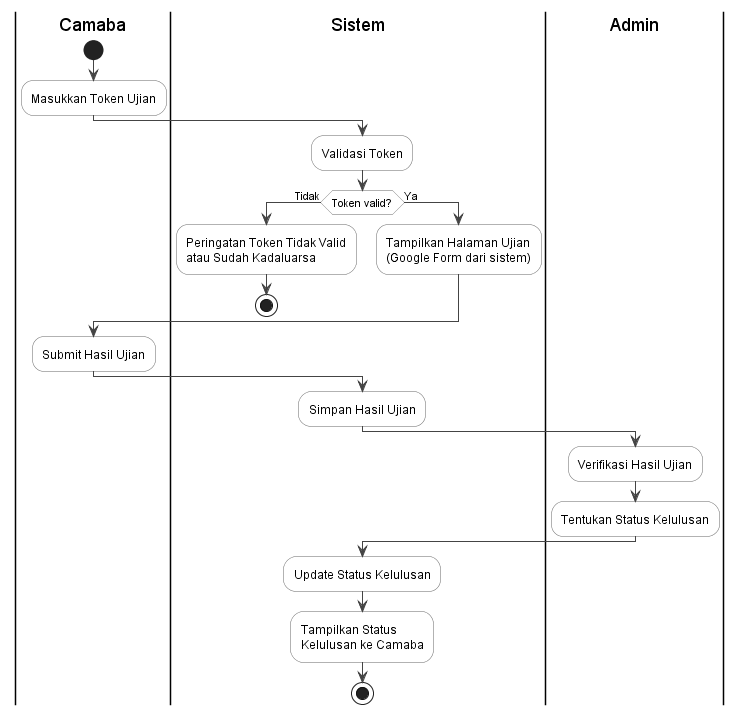
\includegraphics[width=0.85\textwidth]{figure/activity-proses-ujian.png}
	\caption{\textit{Activity} Diagram Proses Ujian Camaba}
	\label{fig:3.activityujian}
\end{figure}

Proses dimulai ketika calon mahasiswa memasukkan token ujian yang telah di-\textit{generate} oleh admin pada sistem. Sistem melakukan validasi untuk memastikan token yang di-\textit{input} benar. Jika tidak sesuai, sistem menampilkan peringatan kesalahan. Bila valid, sistem memeriksa kesesuaian jadwal ujian. Jika waktu ujian belum dimulai, pengguna akan mendapatkan pemberitahuan penundaan. Namun jika sudah sesuai, sistem menampilkan halaman ujian yang memuat Google Form dalam \textit{iframe} atau opsi untuk mengunggah bukti ujian \textit{offline}.\par

Setelah ujian selesai, calon mahasiswa men-\textit{submit} hasil ujian melalui sistem. Admin kemudian melakukan verifikasi hasil dan menentukan status kelulusan. Sistem menampilkan status kelulusan kepada calon mahasiswa melalui \textit{dashboard}.\par

\subsubsection{Permintaan, Validasi, dan Pembayaran Cicilan}

\begin{figure}[H]
	\centering
	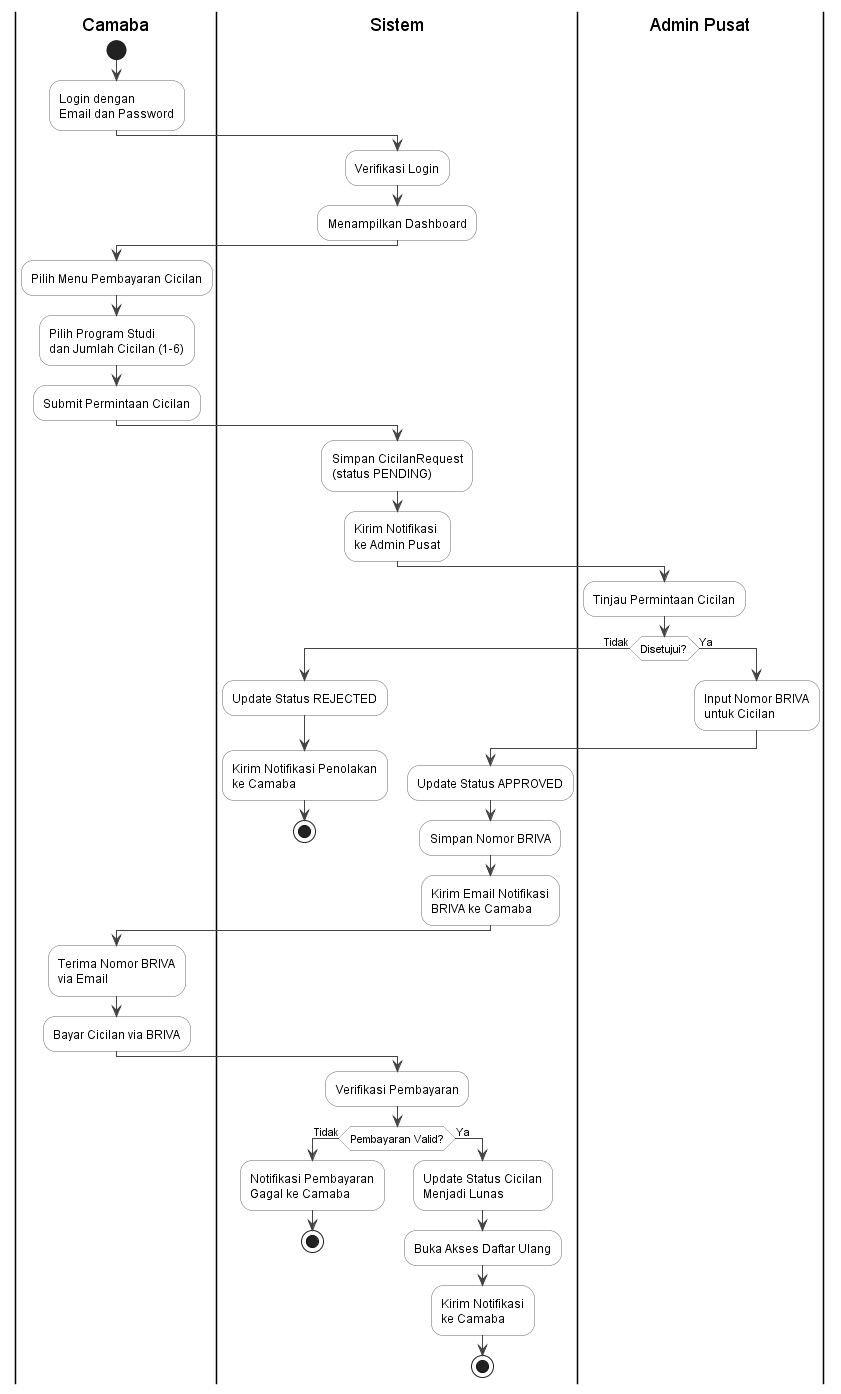
\includegraphics[width=0.85\textwidth]{figure/activity-cicilan.png}
	\caption{\textit{Activity} Diagram Permintaan, Validasi, dan Pembayaran Cicilan}
	\label{fig:3.activitycicilan}
\end{figure}

Proses cicilan dimulai setelah camaba dinyatakan lulus ujian. Camaba login ke sistem, kemudian memilih menu pembayaran cicilan pada \textit{dashboard}. Camaba memilih program studi yang dituju serta jumlah cicilan yang diinginkan, mulai dari 1 hingga 6 tahap sesuai pilihan yang tersedia. Setelah data dikonfirmasi, camaba men-\textit{submit} permintaan cicilan dan sistem menyimpan entri \textit{CicilanRequest} dengan status \textit{PENDING}, kemudian mengirimkan notifikasi ke admin pusat.\par

Admin pusat meninjau permintaan cicilan yang masuk. Jika permintaan ditolak, status diperbarui menjadi \textit{REJECTED} dan sistem mengirimkan notifikasi penolakan beserta alasan ke camaba. Jika disetujui, admin pusat memasukkan nomor Virtual Account BRIVA yang ditetapkan untuk cicilan tersebut, kemudian sistem memperbarui status menjadi \textit{APPROVED} dan mengirimkan email notifikasi berisi nomor BRIVA kepada camaba.\par

Camaba menerima nomor BRIVA melalui email dan melakukan pembayaran cicilan sesuai nominal yang tertera. Sistem kemudian memverifikasi pembayaran. Apabila pembayaran berhasil terverifikasi, sistem memperbarui status cicilan menjadi lunas dan membuka akses menu daftar ulang bagi camaba. Jika pembayaran gagal atau tidak terverifikasi, sistem mengirimkan notifikasi kegagalan kepada camaba.\par

\subsubsection{Daftar Ulang}

\begin{figure}[H]
	\centering
	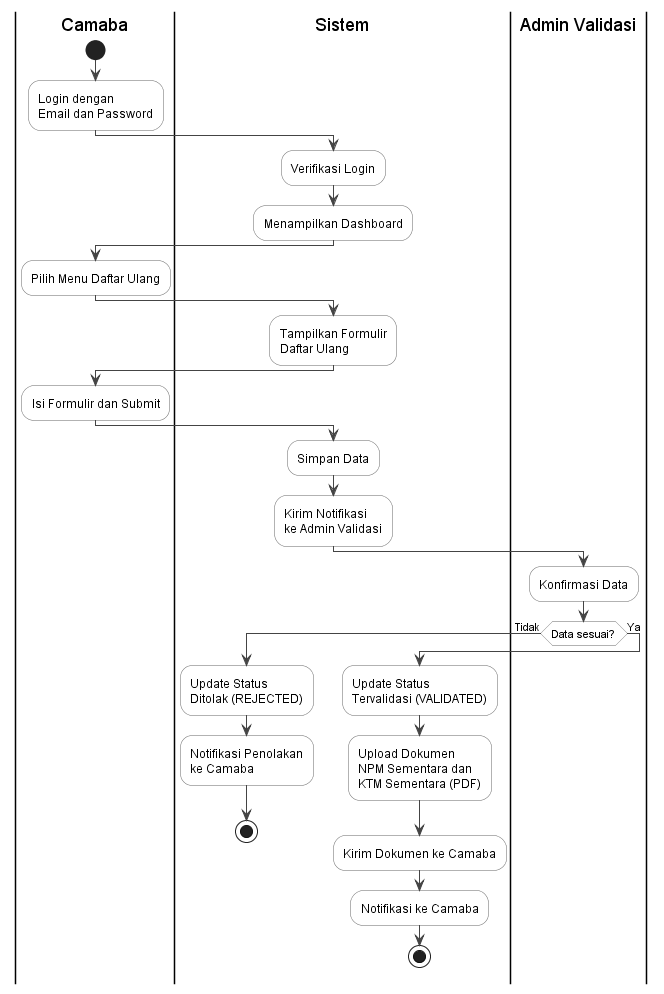
\includegraphics[width=0.85\textwidth]{figure/activity-daftar-ulang.png}
	\caption{\textit{Activity} Diagram Proses Daftar Ulang}
	\label{fig:3.activitydaftarulang}
\end{figure}

Proses dimulai ketika camaba yang lulus login ke sistem menggunakan akun yang telah terdaftar. Setelah masuk, sistem menampilkan \textit{dashboard} dan camaba memilih menu daftar ulang. Sistem menampilkan formulir daftar ulang yang terdiri dari beberapa bagian dokumen yang harus dilengkapi. Setelah semua dokumen diisi dan data dikirim, sistem menyimpan data serta mengirimkan notifikasi ke admin validasi. Admin validasi kemudian melakukan konfirmasi terhadap data daftar ulang. Jika data sudah benar, status dinyatakan terverifikasi dan notifikasi dikirim ke camaba serta admin pusat. Namun, jika data belum sesuai, admin memberikan status ``Perlu Revisi'', dan camaba akan menerima notifikasi untuk memperbaiki data sebelum proses validasi diulang kembali.\par

\subsubsection{Konfigurasi Sistem dan Akun oleh Admin Pusat}

\begin{figure}[H]
	\centering
	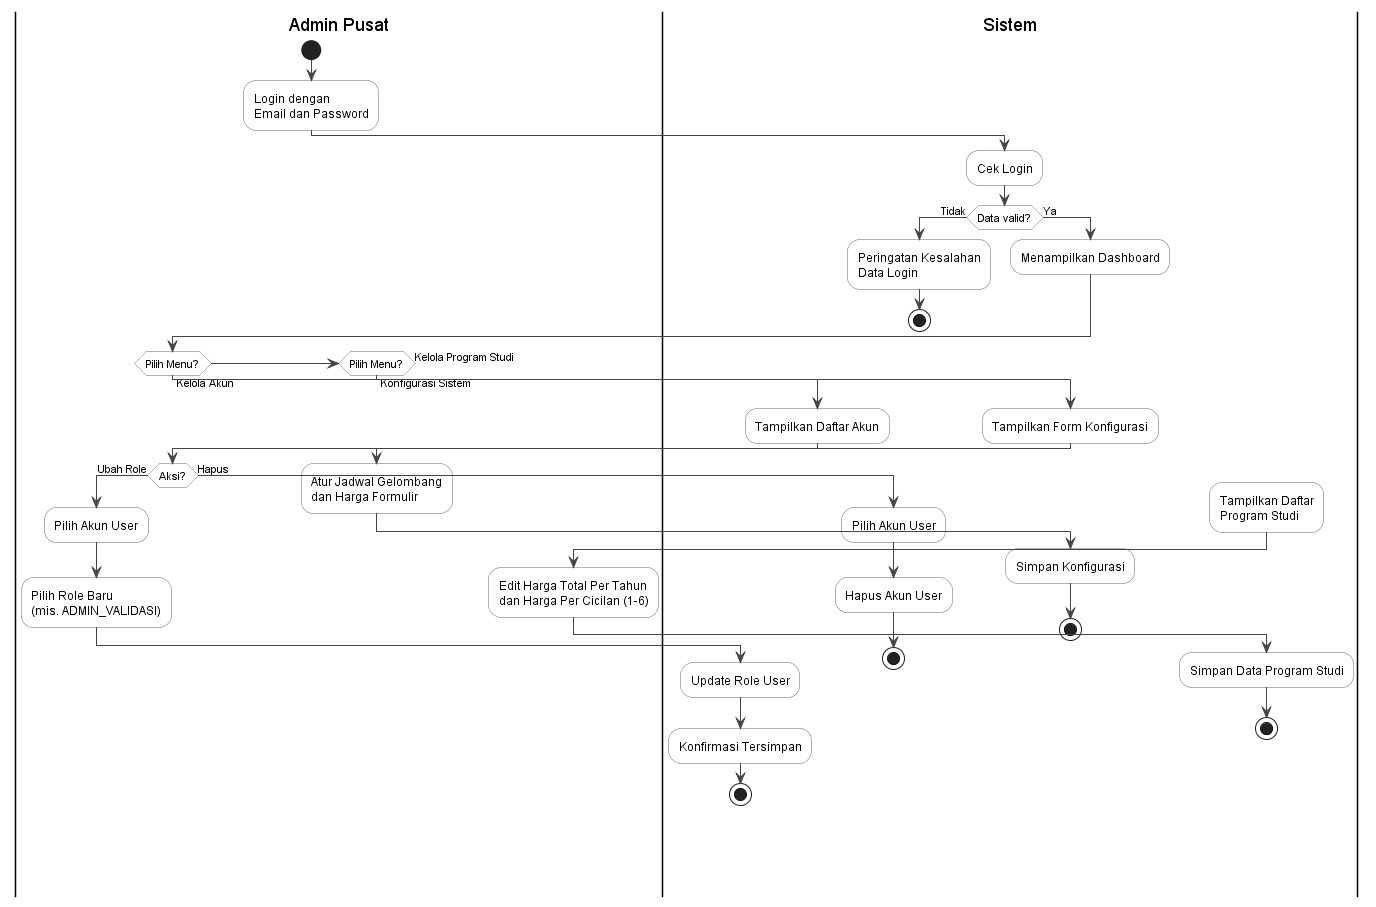
\includegraphics[width=0.85\textwidth]{figure/activity-konfigurasi-admin.png}
	\caption{\textit{Activity} Diagram Konfigurasi Sistem dan Pengelolaan Akun oleh Admin Pusat}
	\label{fig:3.activitykonfigurasi}
\end{figure}

Proses diawali ketika admin pusat melakukan login dengan memasukkan \textit{email} dan \textit{password}. Sistem akan memeriksa data login; jika salah, sistem menampilkan peringatan kesalahan. Jika benar, sistem menampilkan \textit{dashboard} utama. Dari \textit{dashboard}, admin pusat dapat mengelola akun pengguna dengan menekan tombol akun pengguna, menambahkan \textit{user} baru melalui \textit{pop-up} tambah akun, kemudian mengisi \textit{email} dan \textit{password} untuk disimpan ke sistem. Admin juga dapat mengedit atau menghapus akun admin validasi yang sudah ada.\par

Selain itu, admin pusat dapat melakukan konfigurasi sistem, seperti mengatur jadwal gelombang pendaftaran dan menetapkan harga formulir.\par

\subsubsection{Ekspor Data oleh Admin Validasi}

\begin{figure}[H]
	\centering
	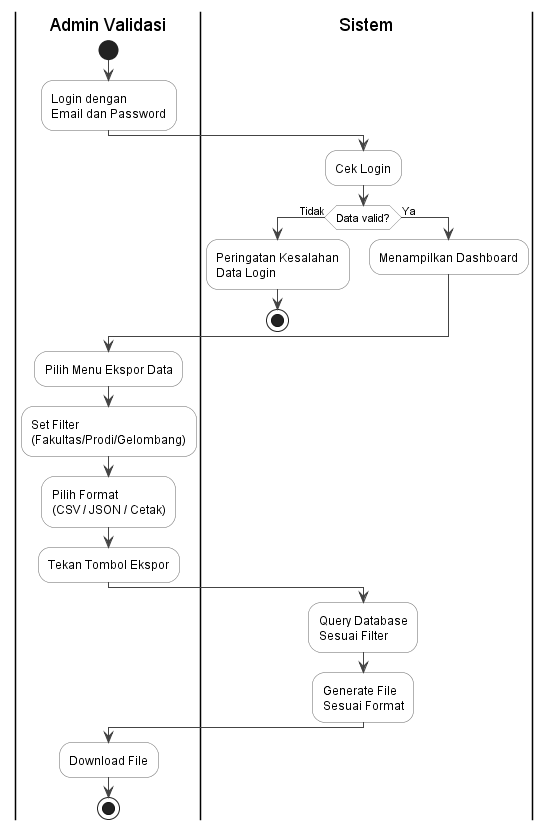
\includegraphics[width=0.85\textwidth]{figure/activity-ekspor-data.png}
	\caption{\textit{Activity} Diagram Ekspor Data oleh Admin Validasi}
	\label{fig:3.activityekspor}
\end{figure}

Proses dimulai ketika admin validasi melakukan login ke sistem dengan memasukkan \textit{email} dan \textit{password}. Sistem akan memeriksa data login; jika salah, sistem menampilkan peringatan kesalahan. Jika benar, sistem menampilkan \textit{dashboard} utama. Dari \textit{dashboard}, admin validasi memilih menu ekspor data dan menentukan filter berdasarkan fakultas, program studi, atau gelombang pendaftaran.\par

Selanjutnya, admin memilih format file ekspor (CSV, JSON, atau Cetak) dan menekan tombol ekspor. Sistem kemudian melakukan \textit{query} pada \textit{database} sesuai dengan filter yang ditetapkan, menghasilkan file dalam format yang dipilih, dan mengunduh file tersebut langsung ke perangkat admin validasi.\par

\subsection{\textit{Sequence} Diagram} \label{III.SequenceDiagram}

\subsubsection{Login dan Registrasi}

\begin{figure}[H]
	\centering
	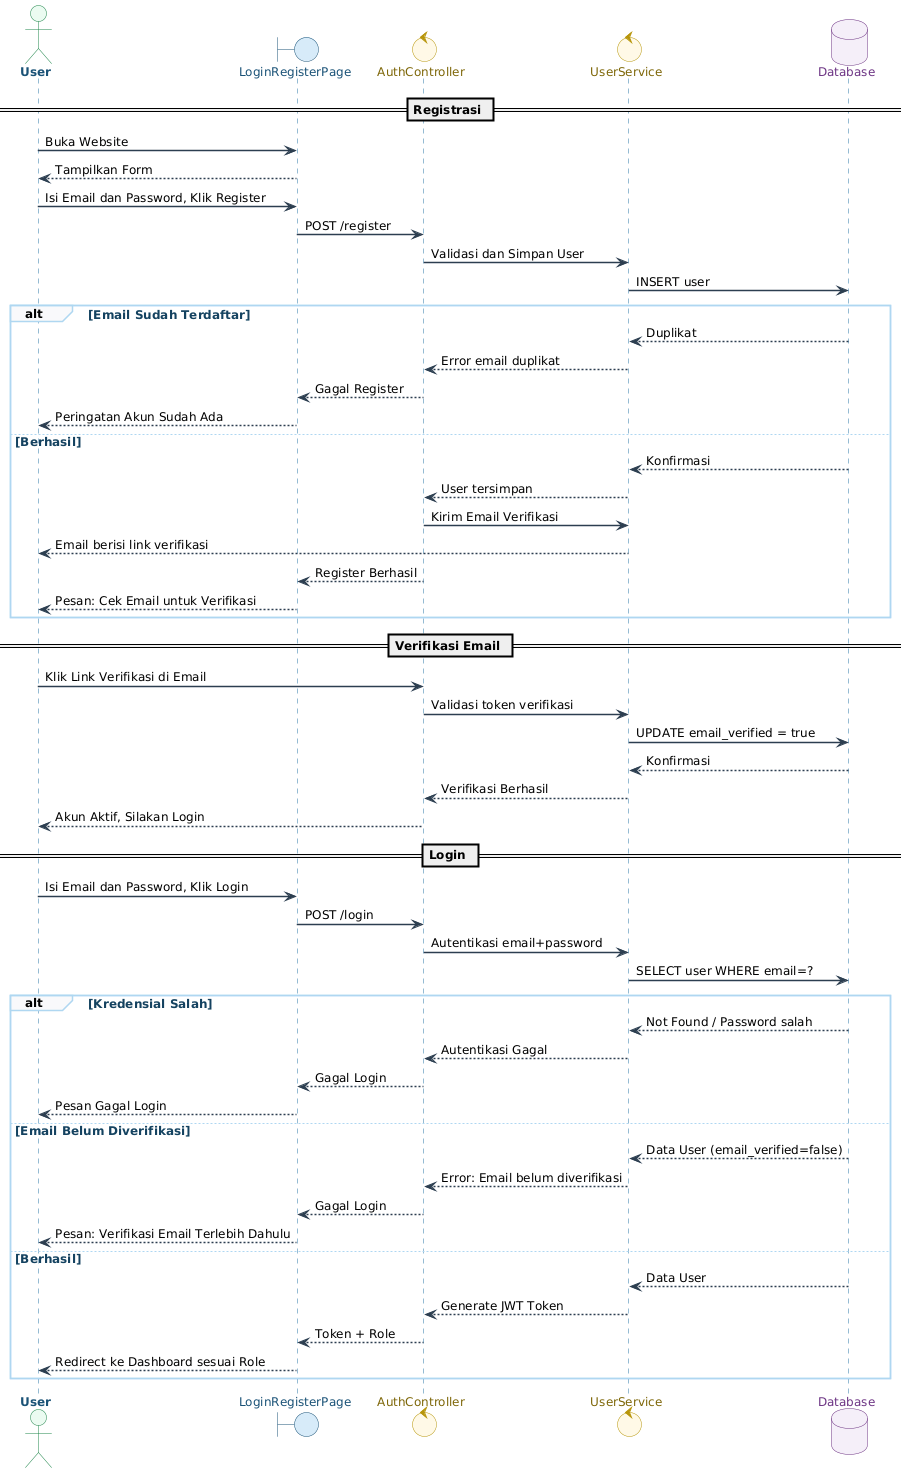
\includegraphics[width=0.85\textwidth]{figure/sequence-user-login.png}
	\caption{\textit{Sequence} Diagram Login dan Registrasi}
	\label{fig:3.sequencelogin}
\end{figure}

Diagram ini menggambarkan alur interaksi antara pengguna, antarmuka sistem, \textit{AuthController}, \textit{UserService}, dan \textit{database} dalam proses registrasi dan login. Pada tahap registrasi, pengguna mengisi email dan kata sandi yang kemudian divalidasi; jika email sudah terdaftar, sistem menampilkan peringatan. Jika berhasil, akun disimpan dan email verifikasi dikirim. Setelah akun diverifikasi, pengguna dapat login menggunakan kredensial yang sama. Sistem memvalidasi data, lalu menghasilkan JWT \textit{token} dan mengarahkan pengguna ke \textit{dashboard} sesuai \textit{role}-nya.\par

\subsubsection{Pendaftaran dan Pengisian Formulir}

\begin{figure}[H]
	\centering
	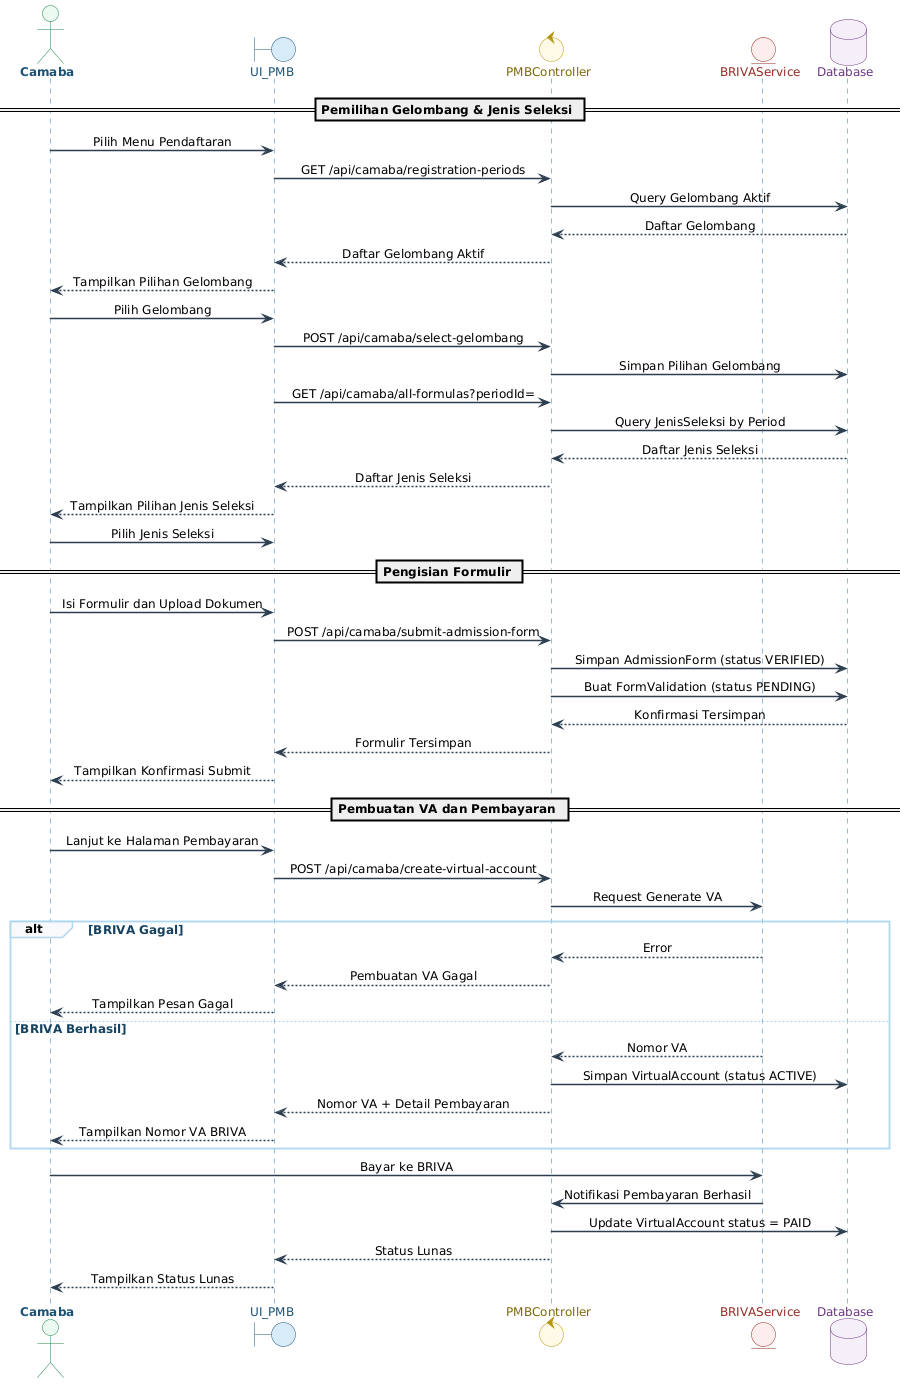
\includegraphics[width=0.85\textwidth]{figure/sequence-pendaftaran-formulir.png}
	\caption{\textit{Sequence} Diagram Pendaftaran dan Pengisian Formulir}
	\label{fig:3.sequenceformulir}
\end{figure}

Diagram ini menggambarkan interaksi antara camaba, antarmuka PMB, \textit{PMBController}, \textit{BRIVAService}, dan \textit{database} dalam proses pendaftaran. Alur dibagi menjadi tiga tahap utama: pemilihan gelombang dan jenis seleksi, pengisian dan pengiriman formulir pendaftaran, serta pembuatan \textit{virtual account} dan pembayaran. Setelah formulir berhasil disimpan dan status \textit{FormValidation} dibuat, camaba mengajukan permintaan pembuatan VA BRIVA. Setelah pembayaran dikonfirmasi oleh BRIVA, status VA diperbarui menjadi PAID.\par

\subsubsection{Proses Ujian}

\begin{figure}[H]
	\centering
	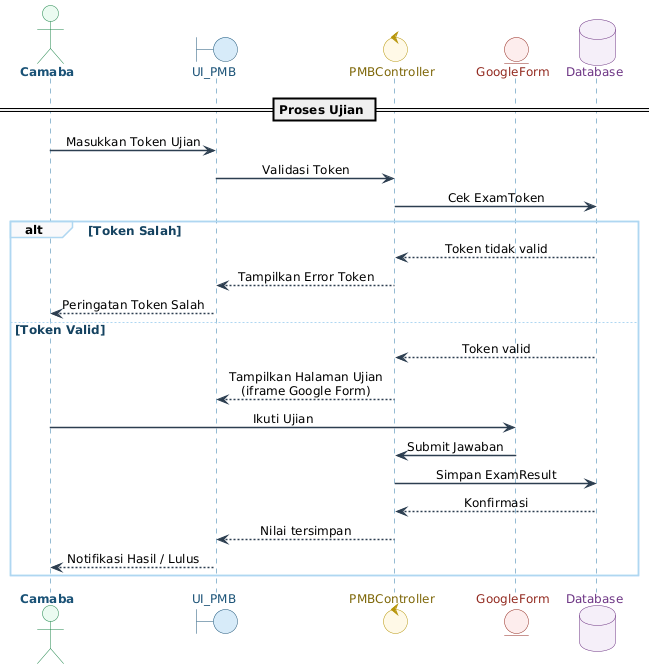
\includegraphics[width=0.85\textwidth]{figure/sequence-pendaftaran-ujian.png}
	\caption{\textit{Sequence} Diagram Proses Ujian}
	\label{fig:3.sequenceujian}
\end{figure}

Diagram ini menggambarkan alur ujian camaba setelah mendapatkan token ujian dari admin melalui email. Camaba memasukkan token melalui antarmuka PMB yang kemudian divalidasi oleh \textit{PMBController} ke \textit{database}. Jika token tidak valid, sistem menampilkan pesan kesalahan. Jika valid, sistem menampilkan halaman ujian yang memuat \textit{Google Form} dalam \textit{iframe}. Setelah ujian selesai dan jawaban dikirim, hasil ujian disimpan ke \textit{database} dan notifikasi dikirim ke camaba.\par

\subsubsection{Daftar Ulang}

\begin{figure}[H]
	\centering
	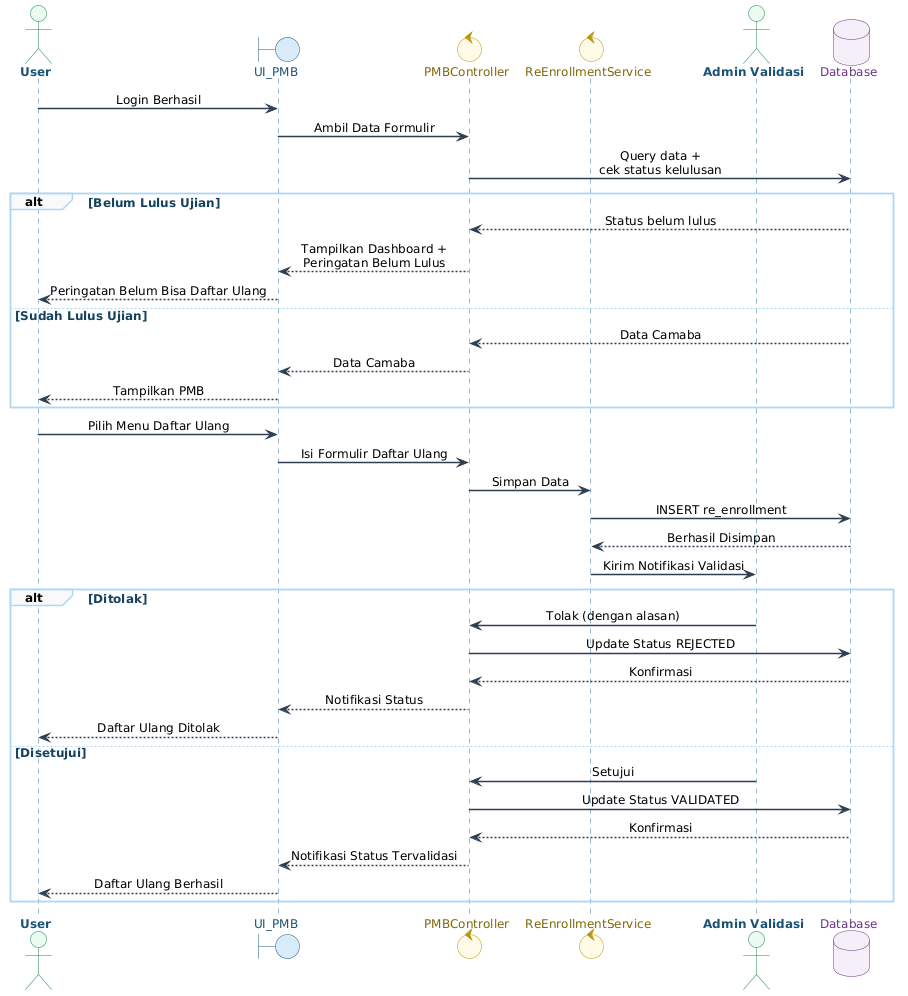
\includegraphics[width=0.85\textwidth]{figure/sequence-daftar-ulang.png}
	\caption{\textit{Sequence} Diagram Proses Daftar Ulang}
	\label{fig:3.sequencedaftarulang}
\end{figure}

Diagram ini menggambarkan alur daftar ulang setelah camaba dinyatakan lulus ujian. Setelah login, sistem memeriksa status kelulusan camaba. Jika belum lulus, sistem menampilkan peringatan. Jika sudah lulus, camaba dapat mengakses menu daftar ulang, mengisi formulir, dan mengirimkan data. Admin validasi menerima notifikasi dan melakukan konfirmasi. Jika ditolak, status diperbarui menjadi REJECTED dan camaba diberitahu. Jika disetujui, status menjadi VALIDATED dan notifikasi keberhasilan dikirim ke camaba.\par

\subsubsection{Validasi Formulir oleh Admin}

\begin{figure}[H]
	\centering
	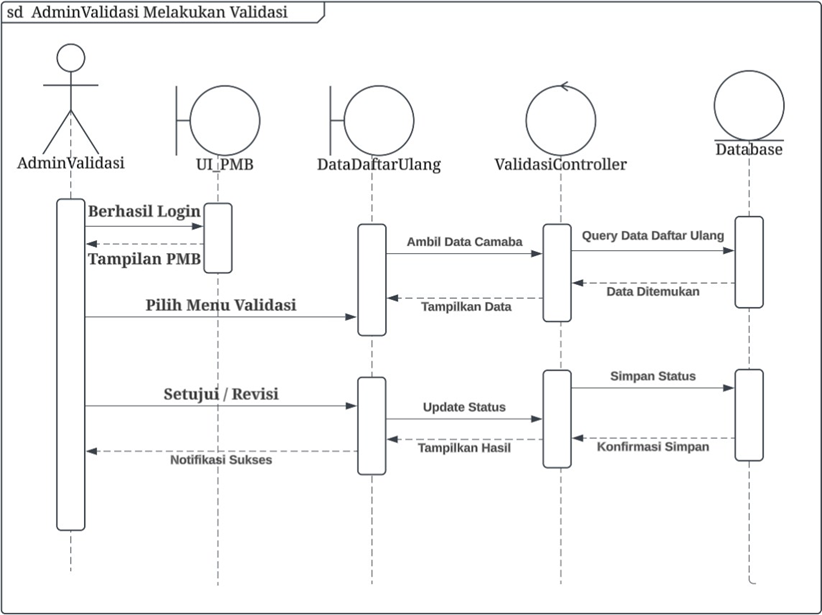
\includegraphics[width=0.85\textwidth]{figure/sequence-validasi.png}
	\caption{\textit{Sequence} Diagram Validasi Formulir oleh Admin}
	\label{fig:3.sequencevalidasi}
\end{figure}

Diagram ini menggambarkan interaksi antara admin validasi, antarmuka sistem, dan \textit{database} dalam proses peninjauan formulir pendaftaran camaba. Admin mengakses daftar formulir yang masuk, memilih salah satu untuk ditinjau, kemudian memutuskan untuk menyetujui atau menolak formulir tersebut. Jika disetujui, sistem memperbarui status validasi menjadi APPROVED dan mengirim token ujian ke camaba melalui email. Jika ditolak, sistem memperbarui status menjadi REJECTED dan mengirim notifikasi beserta alasan penolakan ke camaba.\par

\subsection{\textit{Class} Diagram} \label{III.ClassDiagram}

\begin{figure}[H]
	\centering
	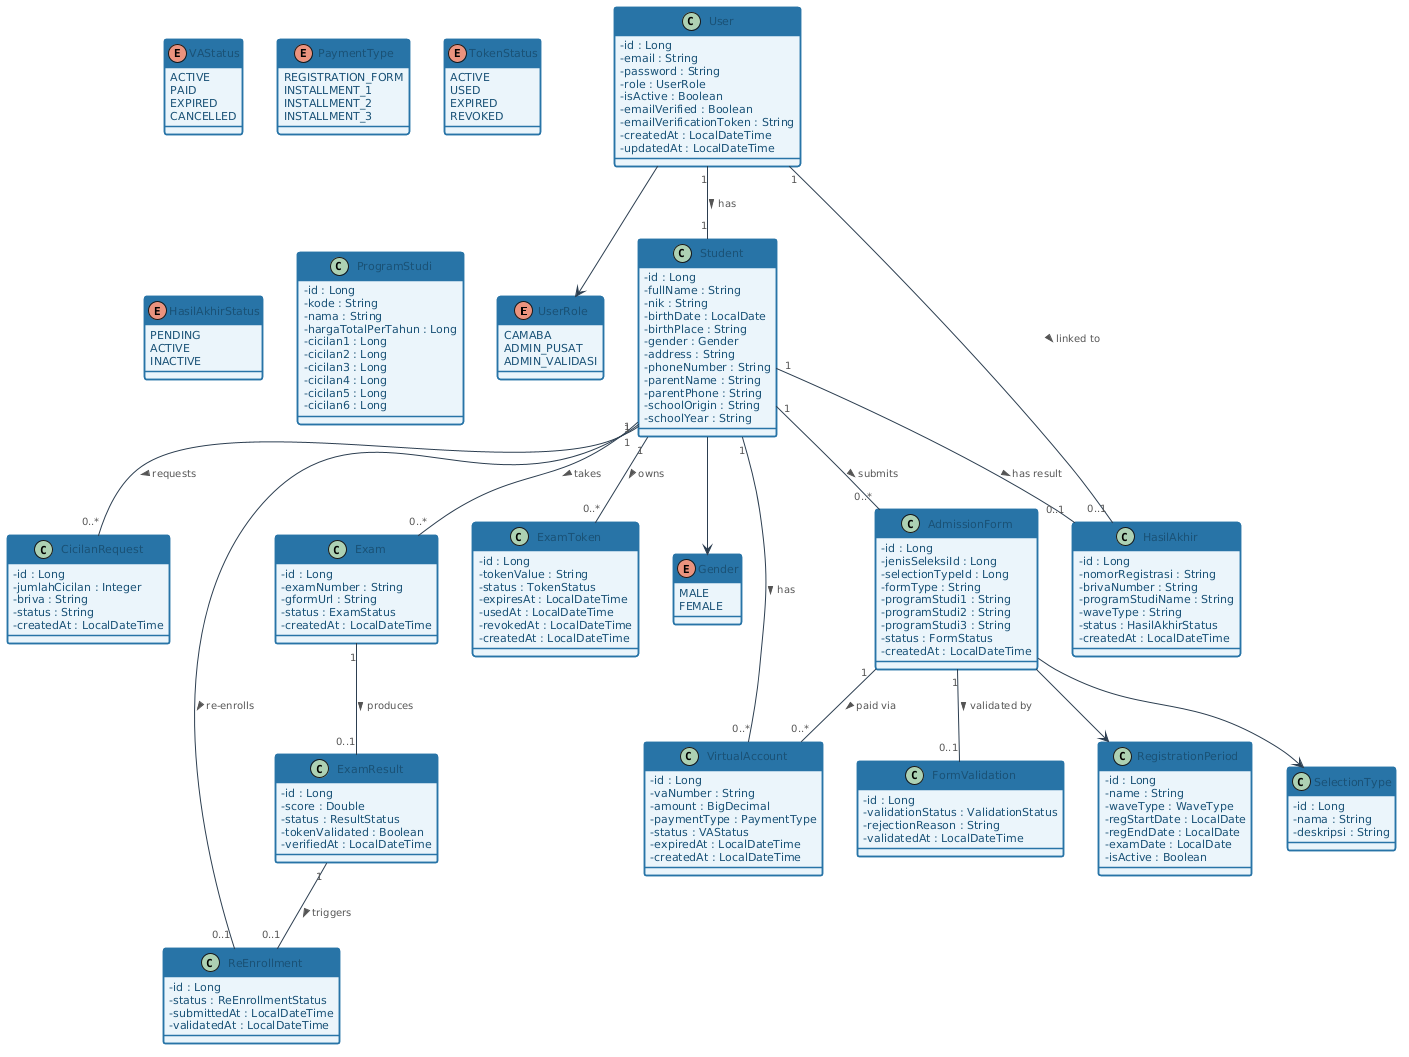
\includegraphics[width=0.85\textwidth]{figure/class-diagram.png}
	\caption{\textit{Class} Diagram}
	\label{fig:3.classdiagram}
\end{figure}

Pada Gambar \ref{fig:3.classdiagram}, \textit{class diagram} sistem PMB UHN menggambarkan struktur entitas utama beserta hubungan antar-kelas. Kelas \texttt{User} merupakan entitas autentikasi pusat dengan atribut \texttt{email}, \texttt{password} (terenkripsi BCrypt), dan \texttt{role}. Tidak ada pewarisan dari \texttt{User}; pembedaan peran dilakukan melalui atribut \texttt{role} bertipe enumerasi \texttt{UserRole} yang memuat tiga nilai: \texttt{STUDENT}, \texttt{ADMIN\_PUSAT}, dan \texttt{ADMIN\_VALIDASI}. Kelas ini mengimplementasikan antarmuka \texttt{UserDetails} dari Spring Security.\par

Profil camaba direpresentasikan oleh kelas \texttt{Student} yang berelasi satu-ke-satu (\textit{one-to-one}) dengan \texttt{User}, menyimpan data pribadi seperti nama, NIK, tempat dan tanggal lahir, alamat, dan asal sekolah. Kelas \texttt{AdmissionForm} mencatat formulir pendaftaran tiap camaba dan berelasi banyak-ke-satu (\textit{many-to-one}) dengan \texttt{Student} serta \texttt{RegistrationPeriod}. Proses verifikasi berkas ditangani oleh \texttt{FormValidation} yang berelasi satu-ke-satu dengan \texttt{AdmissionForm}.\par

Modul ujian dikelola oleh kelas \texttt{Exam}, \texttt{ExamToken}, \texttt{ExamResult}, dan \texttt{ExamSubmission}. Setiap camaba hanya boleh memiliki satu \texttt{Exam} per periode (\textit{one-to-one} antara \texttt{Student} dan \texttt{Exam}). Modul daftar ulang ditangani oleh \texttt{ReEnrollment} yang berelasi satu-ke-satu dengan \texttt{Student}, dan hasilnya dicatat pada \texttt{HasilAkhir}. Sistem pembayaran menggunakan kelas \texttt{VirtualAccount} (integrasi BRIVA) dan \texttt{CicilanRequest} untuk skema cicilan. Kelas pendukung lainnya seperti \texttt{ProgramStudi}, \texttt{GelombangLinkUjian}, \texttt{AdminMessage}, \texttt{SystemLink}, \texttt{ContactInfo}, dan \texttt{Announcement} melengkapi fungsionalitas administrasi dan konfigurasi sistem.\par

\subsection{Diagram Konteks} \label{III.DiagramKonteks}
Diagram konteks berikut menggambarkan hubungan antara Sub-sistem Penerimaan Mahasiswa Baru (PMB) Universitas HKBP Nommensen dengan berbagai entitas eksternal yang terlibat dalam proses PMB. Diagram ini menunjukkan aliran data utama dari dan ke sistem, serta fungsi masing-masing pihak yang berinteraksi.\par

Terdapat lima entitas utama yang berinteraksi langsung dengan sistem:\par
\begin{itemize}[noitemsep]
	\item \textbf{Camaba} (Calon Mahasiswa Baru): Melakukan registrasi, pembelian formulir, pengisian data, mengikuti ujian, daftar ulang, dan menerima hasil seleksi.
	\item \textbf{Admin Pusat}: Mengelola konfigurasi sistem seperti periode penerimaan, jenis seleksi, informasi publik, dan akun admin validasi.
	\item \textbf{Admin Validasi}: Bertugas melakukan validasi data camaba, memverifikasi jalur ranking, mengelola VA manual, serta menolak atau menerima data pendaftaran.
	\item \textbf{BRIVA}: Sebagai sistem eksternal yang digunakan untuk menghasilkan dan memverifikasi \textit{Virtual Account} (VA) secara otomatis.
	\item \textbf{Google Form (GForm)}: Platform eksternal yang digunakan untuk pelaksanaan ujian \textit{online} camaba, diakses melalui \textit{iframe} pada halaman ujian setelah token divalidasi.
\end{itemize}

Setiap entitas terhubung dengan sistem melalui dua jalur data utama: data masuk (\textit{input}) dan data keluar (\textit{output}), yang diringkas dalam panah dengan label masing-masing. Interaksi dirancang agar sesuai dengan prinsip sistem terintegrasi, efisien, dan mudah dikelola oleh seluruh pihak terkait.\par

\begin{figure}[H]
	\centering
	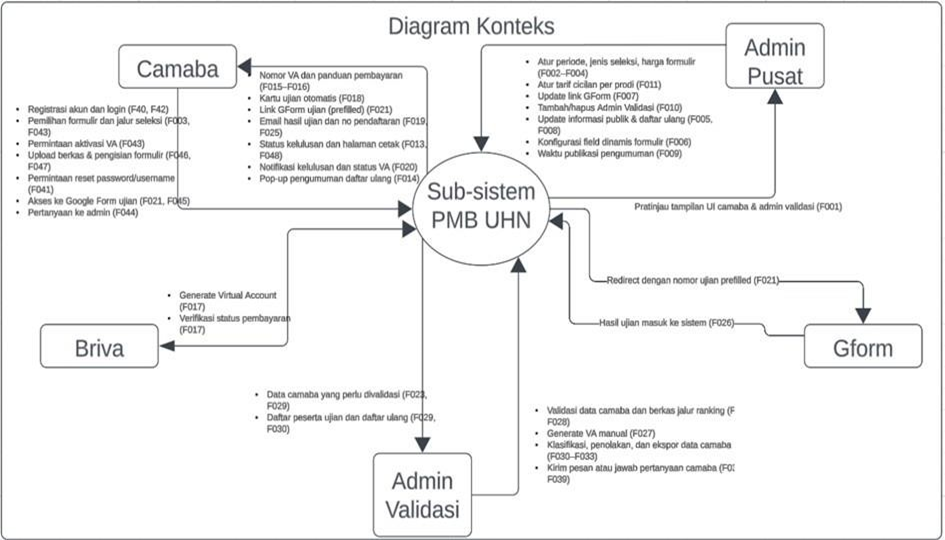
\includegraphics[width=0.85\textwidth]{figure/diagram-konteks.png}
	\caption{Diagram Konteks Sub Sistem Penerimaan Mahasiswa Baru}
	\label{fig:3.diagramkonteks}
\end{figure}

\subsection{ERD (\textit{Entity Relationship Diagram})} \label{III.ERD}

\begin{figure}[H]
	\centering
	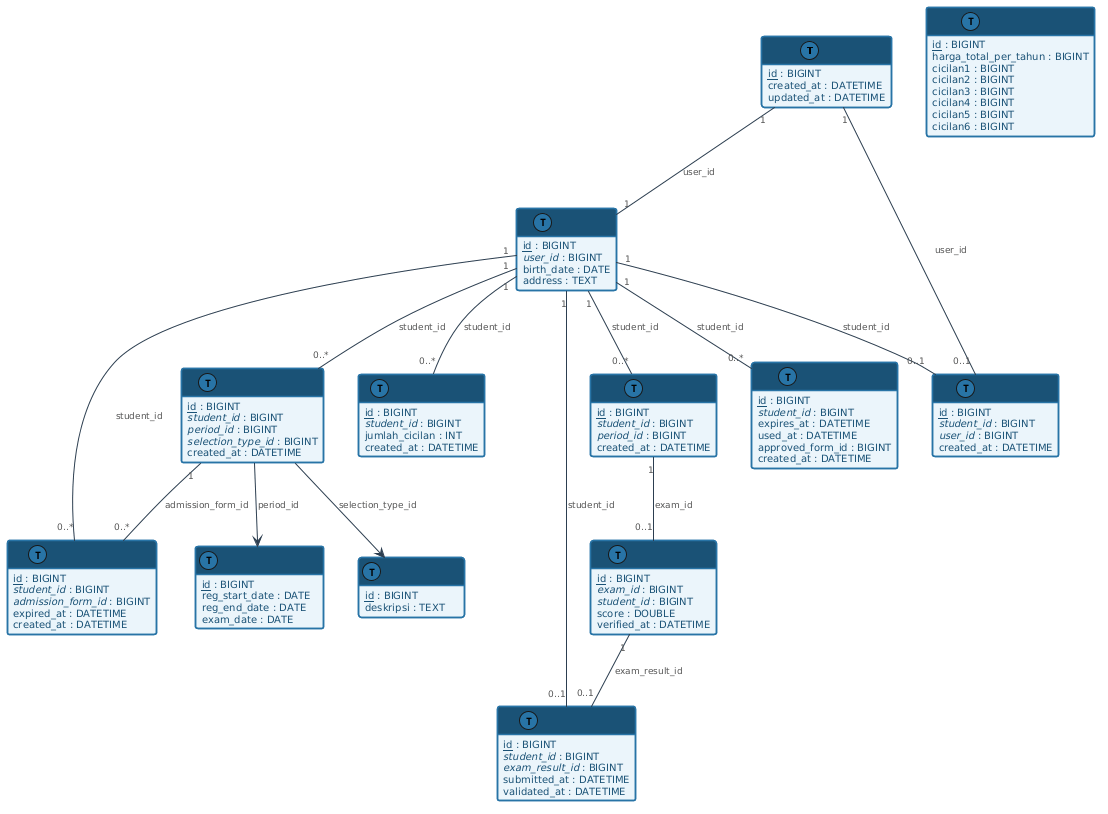
\includegraphics[width=0.85\textwidth]{figure/erd.png}
	\caption{\textit{Entity Relationship Diagram}}
	\label{fig:3.erd}
\end{figure}

ERD sistem penerimaan mahasiswa baru mencakup entitas \texttt{User}, \texttt{Formulir}, \texttt{Periode}, \texttt{ProgramStudi}, \texttt{Pembayaran}, \texttt{Ujian}, \texttt{DaftarUlang}, dan \texttt{Pesan}, dengan hubungan antara \texttt{User} dan \texttt{Formulir}, \texttt{Formulir} dengan \texttt{Pembayaran}, \texttt{Ujian}, serta \texttt{DaftarUlang}, dan juga keterkaitan \texttt{Periode} dan \texttt{ProgramStudi} dengan \texttt{Formulir}. ERD ini memberikan gambaran struktur \textit{database} untuk operasi pendaftaran, pengelolaan data calon mahasiswa baru, serta proses validasi dan pembayaran.\par

\subsection{Rancangan Antarmuka Pengguna} \label{III.RancanganUI}
Rancangan antarmuka pengguna atau \textit{Low-Fidelity Prototype} ini dibuat untuk menggambarkan struktur, alur, dan interaksi utama dalam sistem informasi Penerimaan Mahasiswa Baru (PMB) Universitas HKBP Nommensen. Rancangan ini disusun berdasarkan hasil analisis kebutuhan pengguna.\par

\subsubsection{Halaman Dashboard}
\begin{figure}[H]
	\centering
	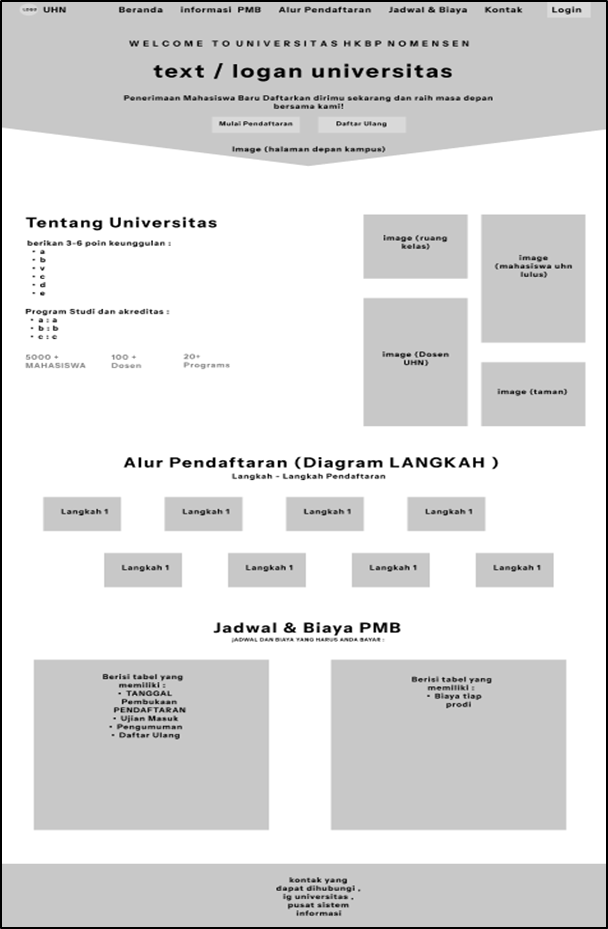
\includegraphics[width=0.75\textwidth]{figure/ui-dashboard.png}
	\caption{Halaman \textit{Dashboard} Calon Mahasiswa Baru}
	\label{fig:3.uidashboard}
\end{figure}
Gambar \ref{fig:3.uidashboard} menunjukkan tampilan \textit{dashboard} camaba, yang menjadi beranda utama setelah pengguna masuk ke sistem. Halaman ini menampilkan ringkasan status pendaftaran, menu navigasi utama, serta informasi umum terkait jadwal dan pengumuman penting.\par

\subsubsection{Halaman Pilih Gelombang Pendaftaran}
\begin{figure}[H]
	\centering
	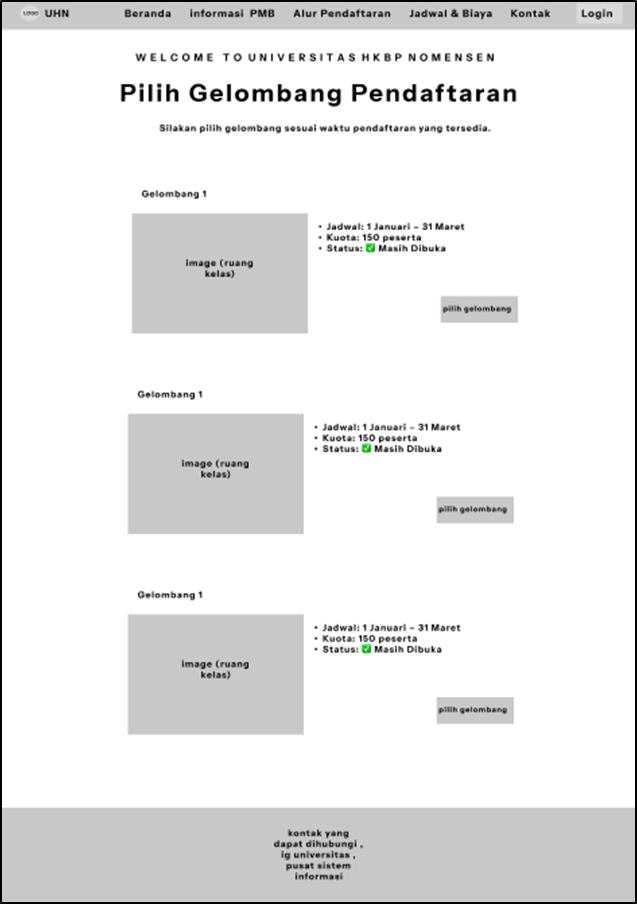
\includegraphics[width=0.75\textwidth]{figure/ui-pilih-gelombang.png}
	\caption{Halaman Pilih Gelombang Pendaftaran}
	\label{fig:3.uipilihgelombang}
\end{figure}
Gambar \ref{fig:3.uipilihgelombang} menampilkan rancangan halaman pemilihan gelombang pendaftaran, tempat camaba memilih gelombang aktif beserta rincian biaya, jadwal, dan batas waktu pendaftaran.\par

\subsubsection{Halaman Pembelian Formulir Pendaftaran}
\begin{figure}[H]
	\centering
	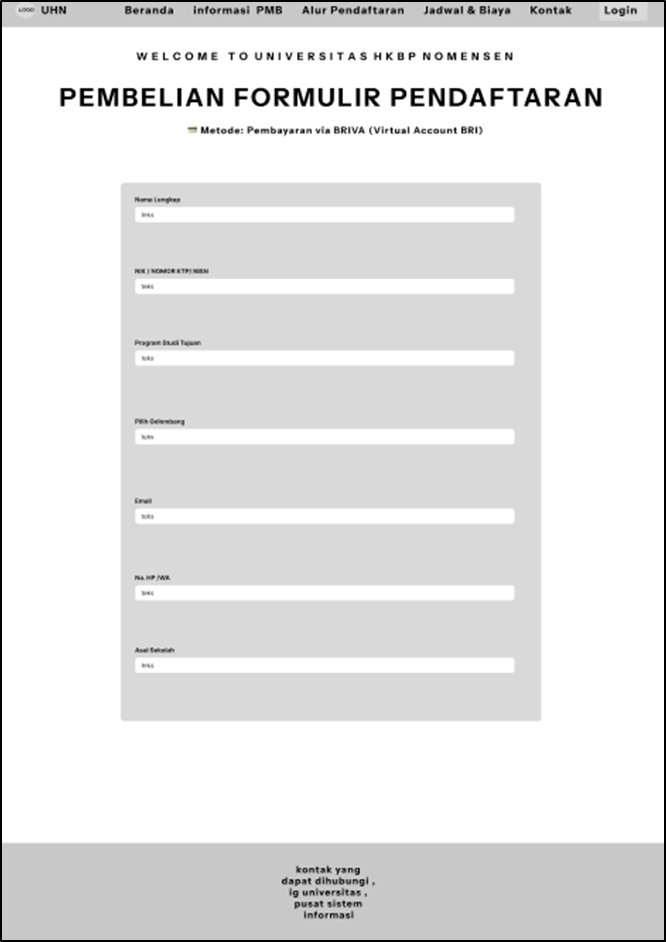
\includegraphics[width=0.75\textwidth]{figure/ui-pembelian-formulir.png}
	\caption{Halaman Pembelian Formulir Pendaftaran}
	\label{fig:3.uipembelianformulir}
\end{figure}
Gambar \ref{fig:3.uipembelianformulir} menampilkan form pembelian formulir pendaftaran, di mana camaba memilih jenis formulir yang tersedia, lalu melanjutkan ke tahap pengisian data dan pembayaran.\par

\subsubsection{Halaman \textit{Pop Out} Rincian Pembayaran}
\begin{figure}[H]
	\centering
	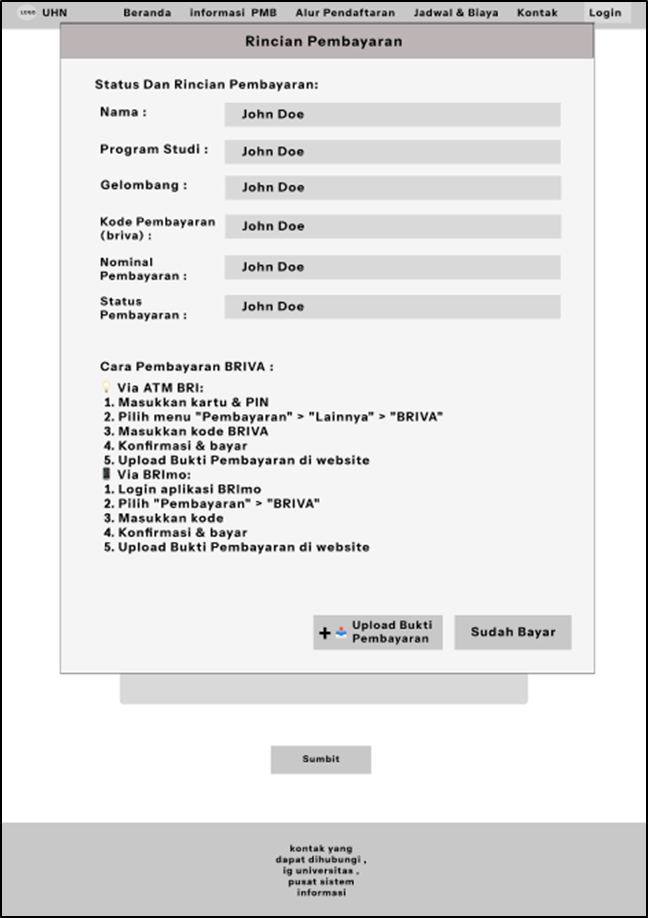
\includegraphics[width=0.75\textwidth]{figure/ui-rincian-pembayaran.png}
	\caption{Halaman \textit{Pop Out} Rincian Pembayaran}
	\label{fig:3.uirincianpembayaran}
\end{figure}
Gambar \ref{fig:3.uirincianpembayaran} menunjukkan \textit{pop-up} rincian pembayaran, yang berfungsi menampilkan detail transaksi seperti kode BRIVA, nominal pembayaran, dan batas waktu pelunasan.\par

\subsubsection{Halaman Status Pembayaran: Diproses}
\begin{figure}[H]
	\centering
	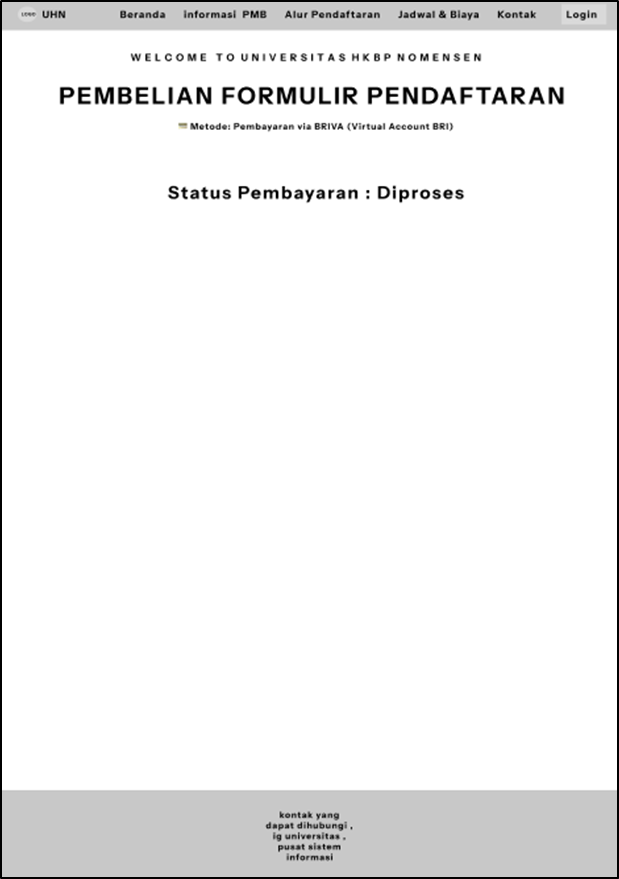
\includegraphics[width=0.75\textwidth]{figure/ui-status-diproses.png}
	\caption{Halaman Status Pembayaran Diproses}
	\label{fig:3.uistatusdiproses}
\end{figure}
Gambar \ref{fig:3.uistatusdiproses} memperlihatkan status pembayaran diproses, di mana sistem sedang menunggu konfirmasi dari server BRIVA.\par

\subsubsection{Halaman Status Pembayaran: Berhasil}
\begin{figure}[H]
	\centering
	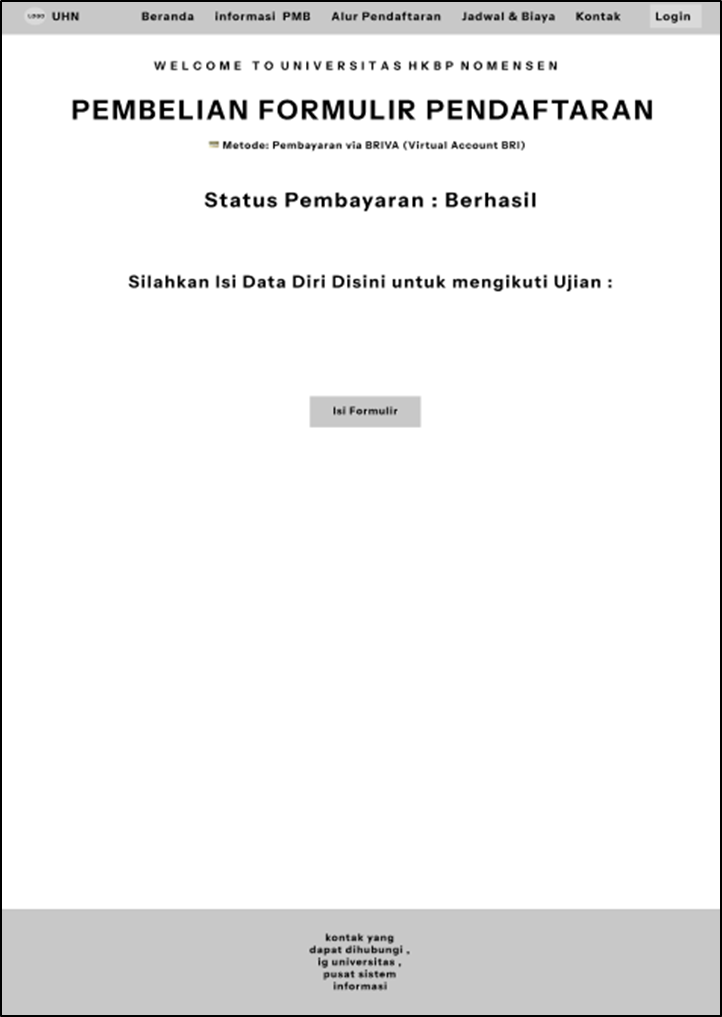
\includegraphics[width=0.75\textwidth]{figure/ui-status-berhasil.png}
	\caption{Halaman Status Pembayaran Berhasil}
	\label{fig:3.uistatusberhasil}
\end{figure}
Gambar \ref{fig:3.uistatusberhasil} menampilkan tampilan status pembayaran berhasil, yang menandakan bahwa pembayaran formulir telah diverifikasi. Setelah status ini muncul, pengguna dapat langsung melanjutkan ke tahap pengisian data diri.\par

\subsubsection{Halaman Pengisian Data Pribadi Formulir}
\begin{figure}[H]
	\centering
	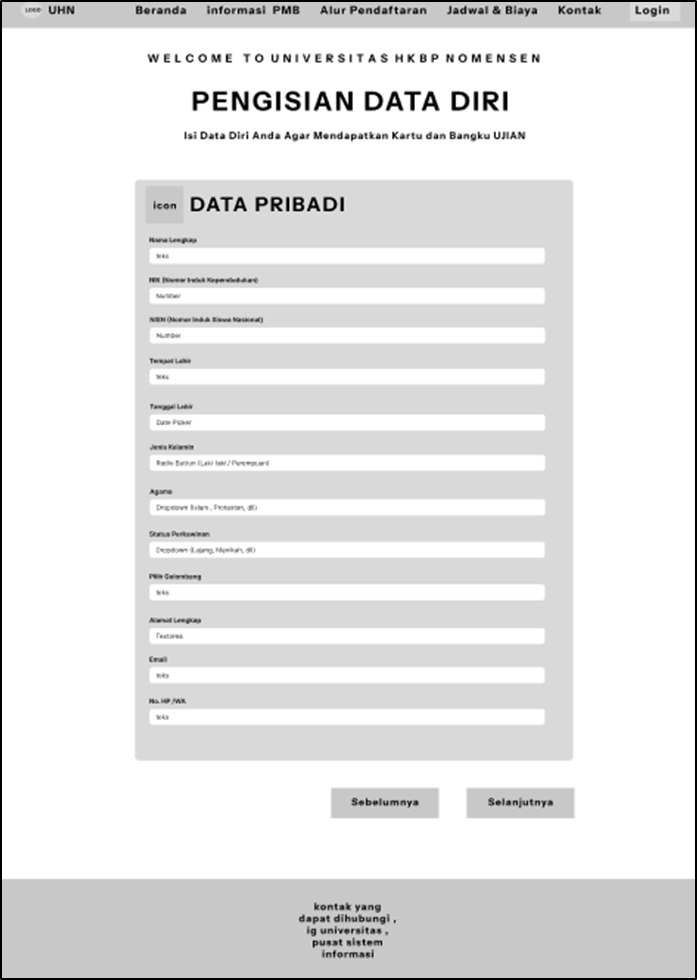
\includegraphics[width=0.75\textwidth]{figure/ui-data-pribadi.png}
	\caption{Halaman Pengisian Data Pribadi Formulir}
	\label{fig:3.uidatapribadi}
\end{figure}
Gambar \ref{fig:3.uidatapribadi} menampilkan form pengisian data pribadi, berisi kolom seperti nama lengkap, NIK, tempat/tanggal lahir, dan jenis kelamin.\par

\subsubsection{Halaman Pengisian Data Diri Pendidikan}
\begin{figure}[H]
	\centering
	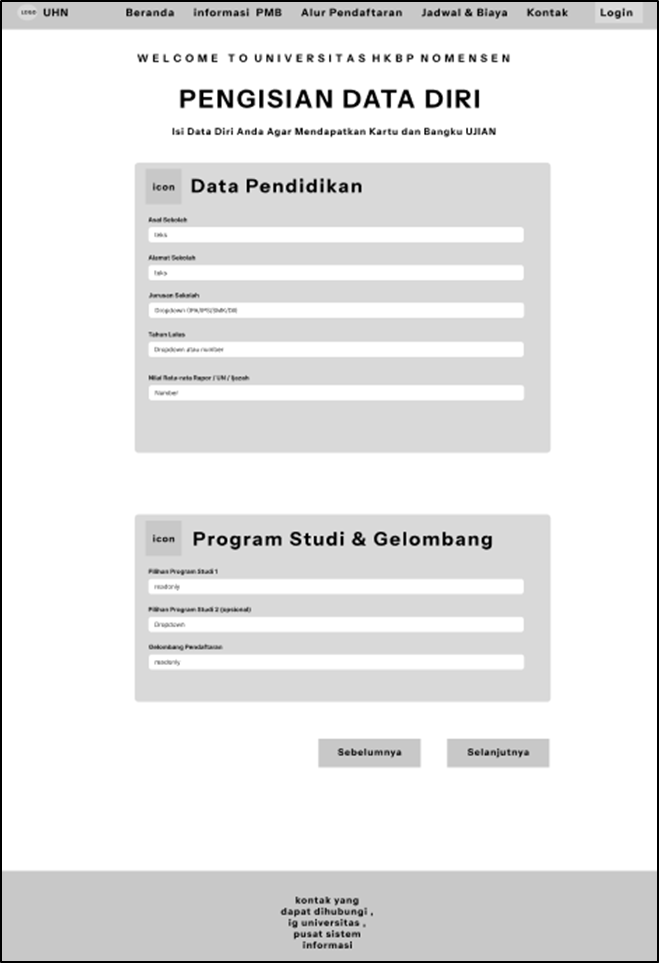
\includegraphics[width=0.75\textwidth]{figure/ui-data-pendidikan.png}
	\caption{Halaman Pengisian Data Diri Pendidikan}
	\label{fig:3.uidatapendidikan}
\end{figure}
Gambar \ref{fig:3.uidatapendidikan} menunjukkan formulir data pendidikan, tempat camaba mengisi informasi asal sekolah, jurusan, dan nilai rata-rata.\par

\subsubsection{Halaman Pengisian Data Wali dan Upload Dokumen}
\begin{figure}[H]
	\centering
	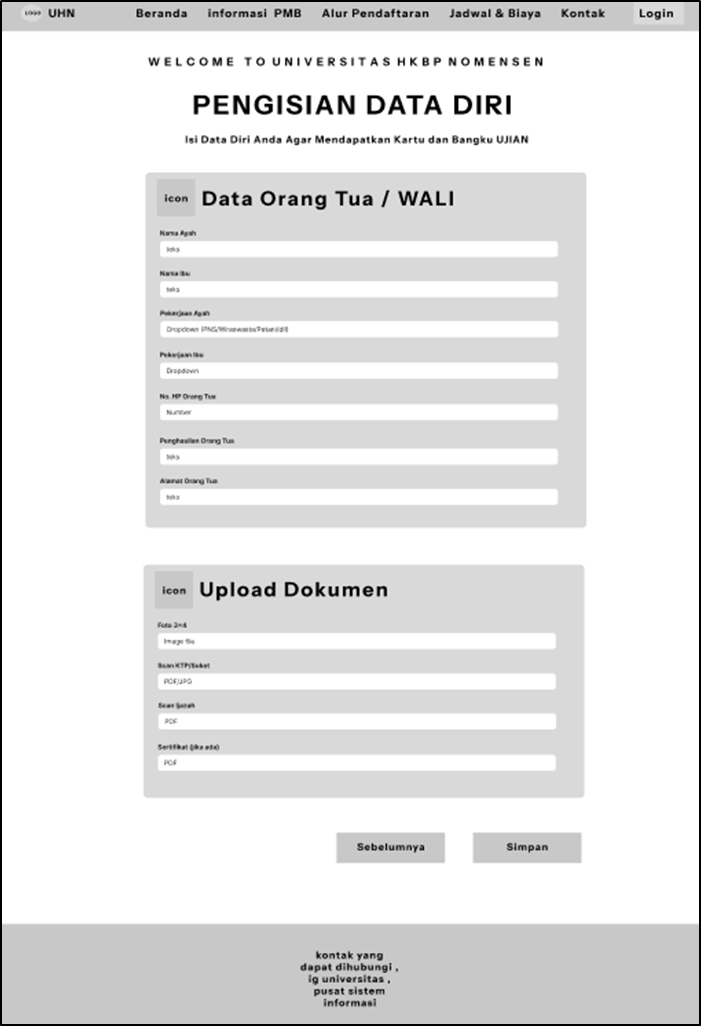
\includegraphics[width=0.75\textwidth]{figure/ui-data-wali.png}
	\caption{Halaman Pengisian Data Wali dan \textit{Upload} Dokumen}
	\label{fig:3.uidatawali}
\end{figure}
Gambar \ref{fig:3.uidatawali} merupakan tampilan form data wali dan unggah dokumen, seperti KTP, ijazah, atau pas foto.\par

\subsubsection{Halaman Kartu Ujian}
\begin{figure}[H]
	\centering
	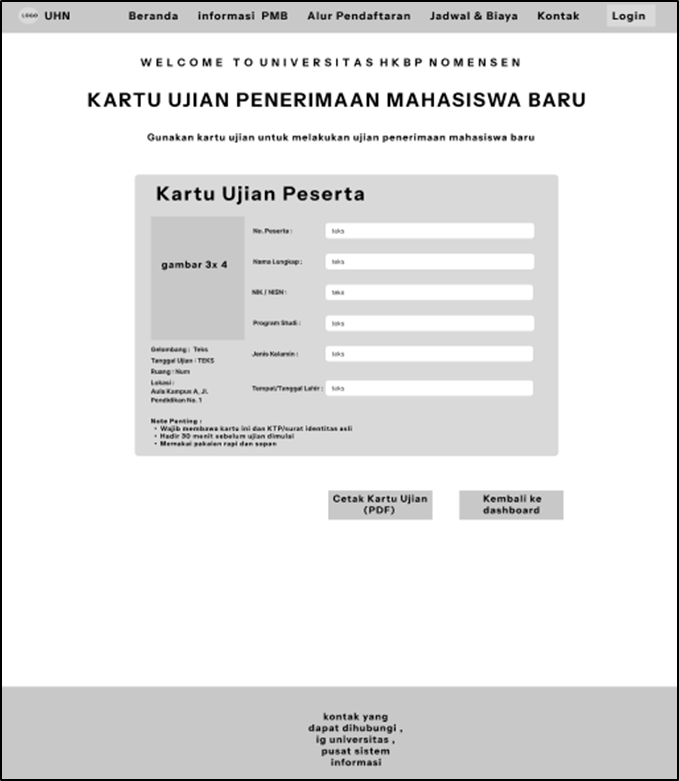
\includegraphics[width=0.75\textwidth]{figure/ui-kartu-ujian.png}
	\caption{Halaman Kartu Ujian}
	\label{fig:3.uikartuujian}
\end{figure}
Gambar \ref{fig:3.uikartuujian} menampilkan kartu ujian otomatis, yang berisi nomor peserta, jadwal, lokasi, serta QR \textit{code} validasi.\par

\subsubsection{Halaman Login Daftar Ulang PMB}
\begin{figure}[H]
	\centering
	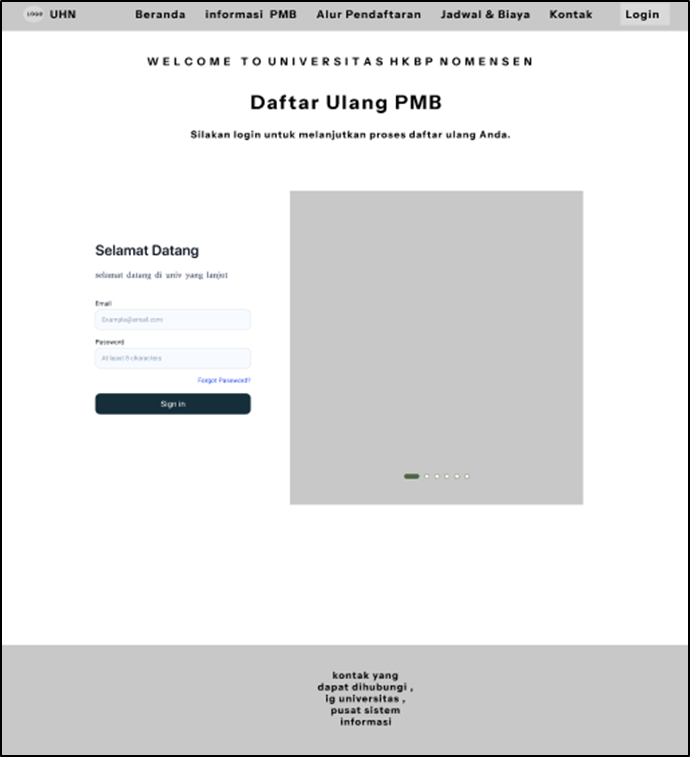
\includegraphics[width=0.75\textwidth]{figure/ui-login-daftar-ulang.png}
	\caption{Halaman Login Daftar Ulang PMB}
	\label{fig:3.uilogindaftarulang}
\end{figure}
Gambar \ref{fig:3.uilogindaftarulang} merupakan rancangan halaman login untuk mengakses daftar ulang, tempat camaba yang telah lulus masuk menggunakan akun reguler yang sama dengan proses pendaftaran.\par

\subsubsection{Halaman Pengisian Data Diri untuk Daftar Ulang}
\begin{figure}[H]
	\centering
	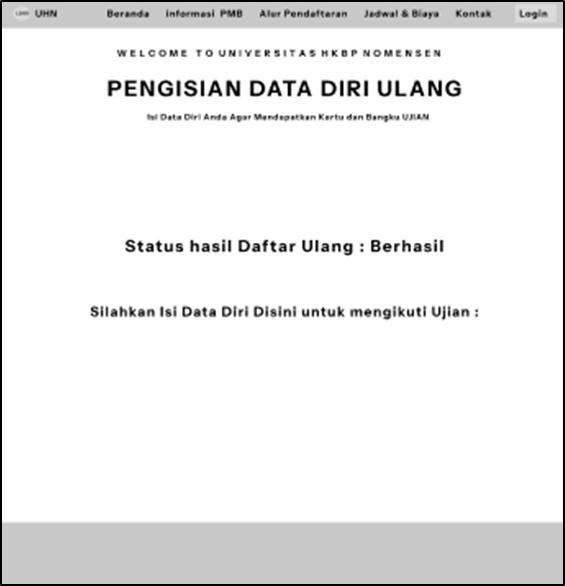
\includegraphics[width=0.75\textwidth]{figure/ui-daftar-ulang.png}
	\caption{Halaman Pengisian Data Diri untuk Daftar Ulang}
	\label{fig:3.uidaftarulang}
\end{figure}
Gambar \ref{fig:3.uidaftarulang} menampilkan formulir daftar ulang, yang menampilkan data lama camaba sekaligus kolom untuk melengkapi informasi tambahan.\par

\subsubsection{Halaman Status Daftar Ulang}
\begin{figure}[H]
	\centering
	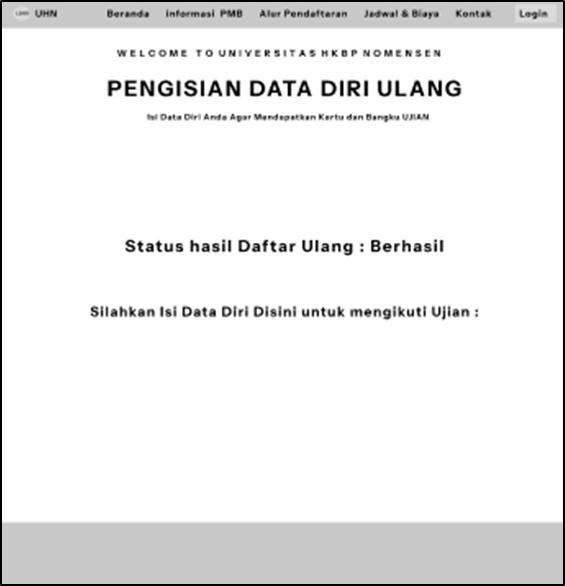
\includegraphics[width=0.75\textwidth]{figure/ui-status-daftar-ulang.png}
	\caption{Halaman Status Daftar Ulang}
	\label{fig:3.uistatusdaftarulang}
\end{figure}
Gambar \ref{fig:3.uistatusdaftarulang} memperlihatkan halaman status daftar ulang, di mana camaba dapat memantau proses validasi oleh admin, mulai dari ``Menunggu'', ``Diterima'', hingga ``Ditolak''.\par

\subsubsection{Halaman Validasi Data Daftar Ulang}
\begin{figure}[H]
	\centering
	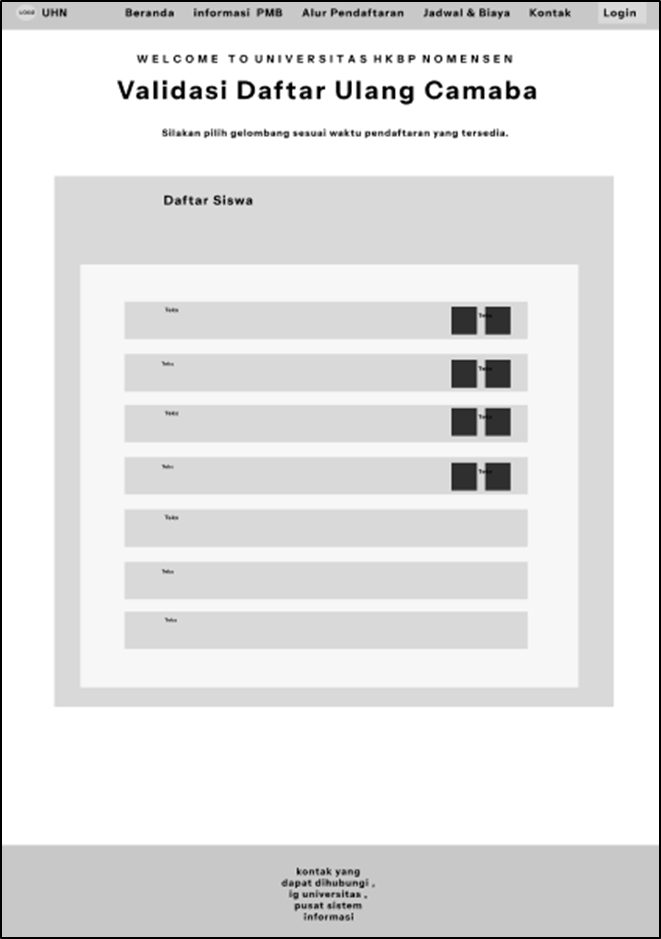
\includegraphics[width=0.75\textwidth]{figure/ui-validasi-daftar-ulang.png}
	\caption{Halaman Validasi Data Daftar Ulang}
	\label{fig:3.uivalidasidaftarulang}
\end{figure}
Gambar \ref{fig:3.uivalidasidaftarulang} merupakan rancangan halaman validasi data daftar ulang yang digunakan oleh admin validasi untuk memeriksa data camaba.\par

\subsubsection{Halaman Kelola Akun User}
\begin{figure}[H]
	\centering
	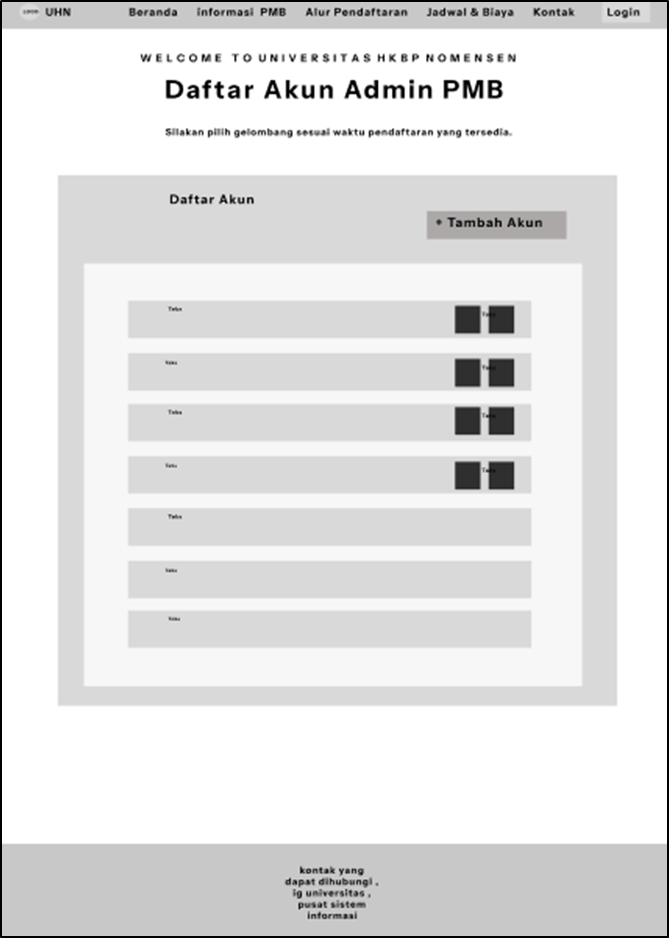
\includegraphics[width=0.75\textwidth]{figure/ui-kelola-akun.png}
	\caption{Halaman Kelola Akun \textit{User}}
	\label{fig:3.uikelolaakun}
\end{figure}
Gambar \ref{fig:3.uikelolaakun} menampilkan halaman kelola akun \textit{user}, yang digunakan oleh admin pusat untuk menambah, menghapus, atau memperbarui akun admin validasi.\par

\section{Pengujian Sistem} \label{III.PengujianSistemRencana}

\subsection{Tujuan Pengujian} \label{III.TujuanPengujian}
Tahap dari pengujian ini adalah untuk memastikan bahwa sistem Penerimaan Mahasiswa Baru (PMB) yang dibangun menggunakan Spring Boot berjalan sesuai dengan fungsionalitas yang telah dirancang. Pengujian dilakukan untuk mengetahui apakah fitur-fitur utama, terutama bagian admin (CMS-\textit{like}) dan \textit{user}, berfungsi dengan benar.\par

\subsection{Jenis Pengujian} \label{III.JenisPengujian}
Pengujian sistem dilakukan menggunakan pendekatan \textit{Black Box Testing}, yaitu dengan memfokuskan pada masukan dan keluaran tanpa memperhatikan struktur kode di dalam sistem.\par

Jenis pengujian yang digunakan:\par
\begin{itemize}[noitemsep]
	\item \textit{Black Box Testing}
	\item Uji Fungsional
	\item Uji Validasi \textit{Input}
	\item Uji Integrasi Modul
\end{itemize}

\subsection{Skema Pengujian Sistem} \label{III.SkemaPengujian}

\subsubsection{Pengujian Fungsional}
\paragraph{\textit{Blackbox Testing}}~\\
Pengujian \textit{blackbox testing} dilakukan untuk menguji kebutuhan fungsional sistem guna memastikan bahwa sistem dapat berjalan dengan semestinya seperti tujuan awal. Pengujian ini memerlukan \textit{input} untuk menghasilkan \textit{output} dan dilakukan pada setiap modul utama. Berikut merupakan parameter untuk mencapai keberhasilan pada fungsional:\par

\begin{longtable}{|p{0.07\textwidth}|p{0.12\textwidth}|p{0.4\textwidth}|p{0.28\textwidth}|}
	\caption{\textit{Blackbox Testing}}
	\label{table:3.blackboxtesting}\\
	\hline
	\textbf{ID} & \textbf{Skenario Pengujian} & \textbf{Deskripsi Pengujian} & \textbf{Hasil yang Diharapkan} \\
	\hline
	\endfirsthead
	\hline
	\textbf{ID} & \textbf{Skenario Pengujian} & \textbf{Deskripsi Pengujian} & \textbf{Hasil yang Diharapkan} \\
	\hline
	\endhead
	TC001 & Login Camaba & Pengguna (Camaba) mengisi form login dengan email dan \textit{password} valid & Pengguna berhasil masuk ke \textit{dashboard} Camaba \\
	\cline{3-4}
	& & Pengguna mengisi form login dengan email dan \textit{password} salah & Sistem menampilkan pesan ``Email atau \textit{Password} salah'' \\
	\hline
	TC002 & Login Gagal & Pengguna mencoba login dengan email benar namun \textit{password} salah & Sistem menolak login dan menampilkan pesan \textit{error} \\
	\cline{3-4}
	& & Pengguna mencoba login dengan email salah namun \textit{password} benar & Sistem menolak login dan menampilkan pesan \textit{error} \\
	\cline{3-4}
	& & Pengguna mencoba login dengan email dan \textit{password} salah & Sistem menolak login dan menampilkan pesan \textit{error} \\
	\hline
	TC003 & Pembelian Formulir & Camaba memilih jalur pendaftaran dan menekan tombol ``Beli'' & Sistem menampilkan \textit{Virtual Account} (VA) dan detail pembayaran \\
	\hline
	TC004 & Kartu Ujian Aktif Setelah Bayar & Camaba mencoba mengakses kartu ujian sebelum melakukan pembayaran & Kartu ujian tidak dapat diakses dan muncul pesan ``Silakan lakukan pembayaran terlebih dahulu'' \\
	\cline{3-4}
	& & Camaba mengakses kartu ujian setelah pembayaran berhasil & Kartu ujian dapat diakses dan diunduh \\
	\hline
	TC005 & Pengisian Data Diri & Camaba mengisi semua data pribadi dengan lengkap lalu menekan tombol Simpan & Data tersimpan dan status berubah menjadi Terkunci \\
	\cline{3-4}
	& & Camaba mencoba menyimpan data yang belum lengkap & Sistem menampilkan pesan ``Lengkapi seluruh data terlebih dahulu'' \\
	\hline
	TC006 & \textit{Upload} Dokumen & Camaba mengunggah file PDF berukuran $<$ 2MB & Dokumen tersimpan dan pratinjau dokumen muncul \\
	\cline{3-4}
	& & Camaba mengunggah file di atas 2MB atau bukan PDF & Sistem menolak \textit{upload} dan menampilkan pesan \textit{error} \\
	\hline
	TC007 & Validasi Admin Menolak Data & Admin menekan tombol ``Tolak'' dan memberikan catatan revisi & Camaba menerima notifikasi penolakan dan bisa mengedit ulang datanya \\
	\hline
	TC008 & Mengikuti Ujian \textit{Online} & Camaba menekan tombol ``Ikuti Ujian'' di \textit{dashboard} & Sistem menampilkan halaman ujian berisi Google Form dalam \textit{iframe} atau opsi unggah bukti ujian \textit{offline} setelah token divalidasi \\
	\hline
	TC009 & Lihat Pengumuman Hasil Ujian & Camaba login setelah ujian selesai & Halaman pengumuman menampilkan status kelulusan sesuai hasil ujian \\
	\hline
	TC010 & \textit{Download} SKL \& Form Daftar Ulang & Camaba menekan tombol ``Unduh'' pada halaman hasil ujian & File PDF SKL dan Formulir Daftar Ulang berhasil diunduh \\
	\hline
\end{longtable}

\paragraph{\textit{Integration Testing}}~\\
Pengujian integrasi dilakukan untuk memastikan setiap modul dalam sistem Penerimaan Mahasiswa Baru (PMB) dapat saling berinteraksi dan bekerja secara menyeluruh sesuai rancangan yang telah dibuat sebelumnya. Tujuan utama pengujian ini adalah memastikan aliran data antar modul berjalan dengan benar serta tidak terjadi kesalahan komunikasi ketika seluruh komponen sistem digabungkan.\par

Pada tahap ini, metode yang digunakan adalah \textit{Black Box Testing}, di mana fokus pengujian bukan pada kode program, melainkan pada hasil keluaran yang dihasilkan dari setiap proses. Tahapan pengujian integrasi meliputi:\par

\begin{enumerate}[noitemsep]
	\item Menggabungkan modul-modul utama yang sebelumnya telah lolos pengujian unit, seperti modul pendaftaran, login, dan \textit{dashboard} admin.
	\item Menjalankan skenario uji berdasarkan urutan proses kerja sistem PMB agar sesuai dengan alur pengguna sebenarnya.
	\item Memastikan data yang dikirim dari satu modul dapat diterima dan diproses dengan benar oleh modul lain.
	\item Mencatat hasil setiap pengujian, termasuk keberhasilan, kesalahan validasi, maupun kemungkinan anomali pada sistem.
\end{enumerate}

Dari hasil pengujian ini diharapkan seluruh modul pada sistem PMB dapat terhubung dan berfungsi dengan baik tanpa menimbulkan kesalahan logika atau gangguan dalam alur proses.\par

\subsubsection{Pengujian Non-Fungsional}
Pengujian non-fungsional dilakukan untuk memastikan bahwa sistem Penerimaan Mahasiswa Baru (PMB) tidak hanya berfungsi dengan baik, tetapi juga memiliki performa, keamanan, dan kemudahan penggunaan yang sesuai dengan harapan pengguna.\par

\begin{longtable}{|p{0.12\textwidth}|p{0.25\textwidth}|p{0.5\textwidth}|}
	\caption{Skenario Uji Kebutuhan Non-Fungsional Sistem PMB}
	\label{table:3.nonfungsional}\\
	\hline
	\textbf{Kebutuhan} & \textbf{Penjelasan} & \textbf{Skenario Uji} \\
	\hline
	\endfirsthead
	\hline
	\textbf{Kebutuhan} & \textbf{Penjelasan} & \textbf{Skenario Uji} \\
	\hline
	\endhead
	\textit{Portability} & Sistem PMB dapat berjalan di berbagai perangkat seperti laptop maupun PC tanpa kendala kompatibilitas. & Pengujian dilakukan dengan mengakses sistem melalui beberapa perangkat dengan sistem operasi berbeda untuk memastikan seluruh fitur berfungsi secara konsisten. \\
	\hline
	\textit{Adaptability} & Sistem dapat diakses melalui berbagai peramban (\textit{web browser}) selama perangkat terhubung ke internet. & Sistem diuji dengan membuka laman PMB melalui Google Chrome, Mozilla Firefox, dan Microsoft Edge. \\
	\hline
	\textit{Reliability} & Sistem diharapkan dapat beroperasi secara stabil tanpa mengalami \textit{crash} atau gangguan server. & Pengujian dilakukan dengan mengakses fitur pendaftaran dan login secara berulang pada waktu berbeda untuk memastikan kestabilan sistem selama digunakan. \\
	\hline
	\textit{Security} & Akses sistem hanya diperbolehkan bagi pengguna dengan akun resmi seperti calon mahasiswa dan admin PMB. & Pengujian dilakukan dengan mencoba proses login menggunakan kombinasi \textit{username} dan \textit{password} yang valid dan tidak valid guna memastikan keamanan autentikasi. \\
	\hline
	\textit{Usability} & Antarmuka dirancang agar mudah dipahami dan digunakan oleh calon mahasiswa maupun admin. & Pengujian dilakukan menggunakan metode \textit{System Usability Scale} (SUS) untuk menilai tingkat kemudahan, kejelasan, dan kenyamanan pengguna dalam proses pendaftaran. \\
	\hline
	\textit{Performance} & Sistem mampu memberikan respons yang cepat terhadap setiap tindakan pengguna. & Pengujian dilakukan dengan mengamati waktu respons sistem secara langsung pada berbagai halaman utama. Sistem dinyatakan baik apabila setiap aksi pengguna memberikan respons dalam waktu kurang dari 5--10 detik. \\
	\hline
\end{longtable}

\paragraph{Pengujian \textit{Usability} (\textit{System Usability Scale} -- SUS)}~\\
Pengujian \textit{usability} menggunakan metode \textit{System Usability Scale} (SUS) bertujuan untuk mengukur sejauh mana sistem PMB mudah digunakan dan memuaskan dari sudut pandang pengguna. Melalui pengujian ini, diperoleh gambaran tentang efektivitas, efisiensi, serta kenyamanan pengguna dalam berinteraksi dengan antarmuka sistem.\par

Metode SUS terdiri dari 10 pernyataan yang dinilai menggunakan skala Likert 1--5, dengan keterangan sebagai berikut:\par

\begin{longtable}{|c|p{0.6\textwidth}|}
	\caption{Penilaian Menggunakan Skala Likert}
	\label{table:3.skalalikert}\\
	\hline
	\textbf{Skor} & \textbf{Keterangan} \\
	\hline
	\endfirsthead
	\hline
	\textbf{Skor} & \textbf{Keterangan} \\
	\hline
	\endhead
	1 & Sangat Tidak Setuju \\
	\hline
	2 & Tidak Setuju \\
	\hline
	3 & Netral \\
	\hline
	4 & Setuju \\
	\hline
	5 & Sangat Setuju \\
	\hline
\end{longtable}

Adapun daftar pernyataan yang digunakan dalam pengujian \textit{usability} ini disajikan pada Tabel \ref{table:3.pernyataansus}.\par

\begin{longtable}{|c|p{0.8\textwidth}|}
	\caption{Daftar Pernyataan \textit{System Usability Scale} (SUS)}
	\label{table:3.pernyataansus}\\
	\hline
	\textbf{No} & \textbf{Pernyataan} \\
	\hline
	\endfirsthead
	\hline
	\textbf{No} & \textbf{Pernyataan} \\
	\hline
	\endhead
	1 & Saya merasa akan sering menggunakan sistem ini. \\
	\hline
	2 & Saya merasa sistem ini rumit untuk digunakan. \\
	\hline
	3 & Saya merasa sistem ini mudah digunakan. \\
	\hline
	4 & Saya memerlukan bantuan dari orang lain atau teknisi untuk dapat menggunakan sistem ini. \\
	\hline
	5 & Saya merasa fitur-fitur dalam sistem ini terintegrasi dengan baik. \\
	\hline
	6 & Saya merasa terdapat inkonsistensi dalam sistem ini. \\
	\hline
	7 & Saya merasa sebagian besar orang akan mudah mempelajari cara menggunakan sistem ini dengan cepat. \\
	\hline
	8 & Saya merasa sistem ini sulit untuk digunakan. \\
	\hline
	9 & Saya merasa percaya diri dalam menggunakan sistem ini. \\
	\hline
	10 & Saya perlu mempelajari banyak hal terlebih dahulu sebelum dapat menggunakan sistem ini. \\
	\hline
\end{longtable}

Dalam proses pengujian, setiap responden memberikan skor berdasarkan pengalaman mereka menggunakan sistem PMB.\par
